%%%%%%%%%%%%%%%%%%%%%%%%%%%%%%%%%%%%%%%%%
% Beamer Presentation
% LaTeX Template
% Version 1.0 (10/11/12)
%
% This template has been downloaded from:
% http://www.LaTeXTemplates.com
%
% License:
% CC BY-NC-SA 3.0 (http://creativecommons.org/licenses/by-nc-sa/3.0/)
%
%%%%%%%%%%%%%%%%%%%%%%%%%%%%%%%%%%%%%%%%%

%----------------------------------------------------------------------------------------
%	PACKAGES AND THEMES
%----------------------------------------------------------------------------------------

\documentclass{beamer}
\newcounter{saveenumi}
\newcommand{\seti}{\setcounter{saveenumi}{\value{enumi}}}
\newcommand{\conti}{\setcounter{enumi}{\value{saveenumi}}}
\mode<presentation> {

% The Beamer class comes with a number of default slide themes
% which change the colors and layouts of slides. Below this is a list
% of all the themes, uncomment each in turn to see what they look like.

%\usetheme{default}
%\usetheme{AnnArbor}
%\usetheme{Antibes}
%\usetheme{Bergen}
%\usetheme{Berkeley}
%\usetheme{Berlin}
%\usetheme{Boadilla}
%\usetheme{CambridgeUS}
%\usetheme{Copenhagen}
%\usetheme{Darmstadt}
%\usetheme{Dresden}
%\usetheme{Frankfurt}
%\usetheme{Goettingen}
%\usetheme{Hannover}
%\usetheme{Ilmenau}
%\usetheme{JuanLesPins}
%\usetheme{Luebeck}
\usetheme{Madrid}
%\usetheme{Malmoe}
%\usetheme{Marburg}
%\usetheme{Montpellier}
%\usetheme{PaloAlto}
%\usetheme{Pittsburgh}
%\usetheme{Rochester}
%\usetheme{Singapore}
%\usetheme{Szeged}
%\usetheme{Warsaw}

% As well as themes, the Beamer class has a number of color themes
% for any slide theme. Uncomment each of these in turn to see how it
% changes the colors of your current slide theme.

%\usecolortheme{albatross}
%\usecolortheme{beaver}
%\usecolortheme{beetle}
%\usecolortheme{crane}
%\usecolortheme{dolphin}
%\usecolortheme{dove}
%\usecolortheme{fly}
%\usecolortheme{lily}
%\usecolortheme{orchid}
%\usecolortheme{rose}
%\usecolortheme{seagull}
%\usecolortheme{seahorse}
%\usecolortheme{whale}
%\usecolortheme{wolverine}

%\setbeamertemplate{footline} % To remove the footer line in all slides uncomment this line
%\setbeamertemplate{footline}[page number] % To replace the footer line in all slides with a simple slide count uncomment this line

%\setbeamertemplate{navigation symbols}{} % To remove the navigation symbols from the bottom of all slides uncomment this line
}

\usepackage{graphicx} % Allows including images
\usepackage{mathrsfs}
\usepackage{booktabs} % Allows the use of \toprule, \midrule and \bottomrule in tables
\usepackage{amsmath}
%----------------------------------------------------------------------------------------
%	TITLE PAGE
%----------------------------------------------------------------------------------------

\title[Sun-Avoidance Slew (SAS) Maneuver ]{Sun-Avoidance Slew (SAS) Maneuver with Single Payload } % The short title appears at the bottom of every slide, the full title is only on the title page

\author{Mohammad Ayoubi} % Your name
%\institute[UCLA] % Your institution as it will appear on the bottom of every slide, may be shorthand to save space
%{
%Space Systems Loral \\ % Your institution for the title page
%
%}
\date{\today} % Date, can be changed to a custom date


\begin{document}
\begin{frame}
  \titlepage
\end{frame}


%-------------------------------------------------------------------------------------------------------------------------------------------------------------------
\begin{frame}
\begin{block}{Sun-Avoidance Slew (SAS) Maneuver}
{\bf Problem Statement:}\\
Given:$_N\hat{P}_i$, $_N\hat{P}_f$, $_N\hat{S}$, $_G\hat{P}$, $\epsilon_p$, $^Nq^G$, $^N_G\omega^G(t_i)$, and $^N_G\omega^G(t_f)$ .\\
%Assumption: The spacecraft is rigid.\\
Find: 
\begin{enumerate}
\item A sequence of slew maneuvers to avoid sun vector.
\item the commanded angular velocity, angular acceleration, and quaternion profiles.
\end{enumerate} 
\end{block}
%\begin{minipage}{0.95\textwidth}
%\begin{center}
%\includegraphics[width=2.25in]{./SAS_Schematic}      
%\end{center}
%\end{minipage}
\begin{figure}
\includegraphics[width=2in]{./Figures/SAS_Schematic}
\caption{The spacecraft is not drawn to scale.}
\end{figure}
\end{frame}
%-------------------------------------------------------------------------------------------------------------------------------------------------------------------
\begin{frame}
\begin{block}{Sun-Avoidance Slew (SAS) Maneuver}
\begin{figure}
\includegraphics[width=3in]{./Figures/SAS_Schematic}
\caption{The spacecraft is not drawn to scale.}
\end{figure}
\end{block}
\end{frame}
%-------------------------------------------------------------------------------------------------------------------------------------------------------------------
\begin{frame}
\begin{block}{Nomenclature}
\begin{itemize}
\item $G$ frame: Unit sphere attached to the gyrostat.
\item $N$: frame: The Newtonian frame fixed in the inertial space.
\item $_G\hat{P}$: Unit vector along the bore sight of payload in the $G$ frame.
\item $_N\hat{P}_i$: Unit vector of the initial point in the $G$ frame.
\item $_N\hat{P}_f$: Unit vector of the final point in the $G$ frame.
\item $_N\hat{S}$: Unit vector of the sun vector in the $N$ frame.
 \item $\epsilon_p$: Payload half-cone angle.
\end{itemize}
\end{block}
\end{frame}

%-------------------------------------------------------------------------------------------------------------------------------------------------------------------
\begin{frame}
\begin{block}{Check the Sun Vector Intrusion}
\begin{enumerate}
\item Check the angular separation between the sun vector, $\hat{S}$, and the $\hat{P}_i-\hat{P}_f$ plane.
\begin{equation}
\alpha=\frac{\pi}{2}-\cos^{-1}(\hat{S}.\hat{e})
\end{equation}
where the eigenaxis is determined by
\begin{equation}\label{eaxis}
\hat{e}=\frac{\hat{P}_i\times\hat{P}_f}{|\hat{P}_i\times \hat{P}_f|}
\end{equation} 

\item IF $|\alpha|<\epsilon_p$,THEN determine the projection of the sun vector into the $\hat{P}_i-\hat{P}_f$ plane.
\begin{equation}\label{Sbar}
\vec{S}_{||}=\hat{S}\cos\alpha
\end{equation}

\end{enumerate}
\end{block}
\end{frame}

%-------------------------------------------------------------------------------------------------------------------------------------------------------------------
\begin{frame}
\begin{block}{Slew Maneuvers}
\begin{enumerate}
\item The $1^{st}$ slew around the eigenaxis,$\hat{e}$, through angle:
\end{enumerate}
 \begin{equation}
 \phi_1=\left\{
                \begin{array}{ll}
                 \cos^{-1}(\hat{P}._G\hat{S}_{||})-\epsilon_p& when\  \cos^{-1}(\hat{P}._G\hat{S}_{||})-\epsilon_p\leq \pi\\
                 \cos^{-1}(\hat{P}._G\hat{S}_{||})-\epsilon_p-2\pi& when\ \cos^{-1}(\hat{P}._G\hat{S}_{||})-\epsilon_p>\pi\\
                \end{array}
              \right.
 \end{equation}
\begin{figure}
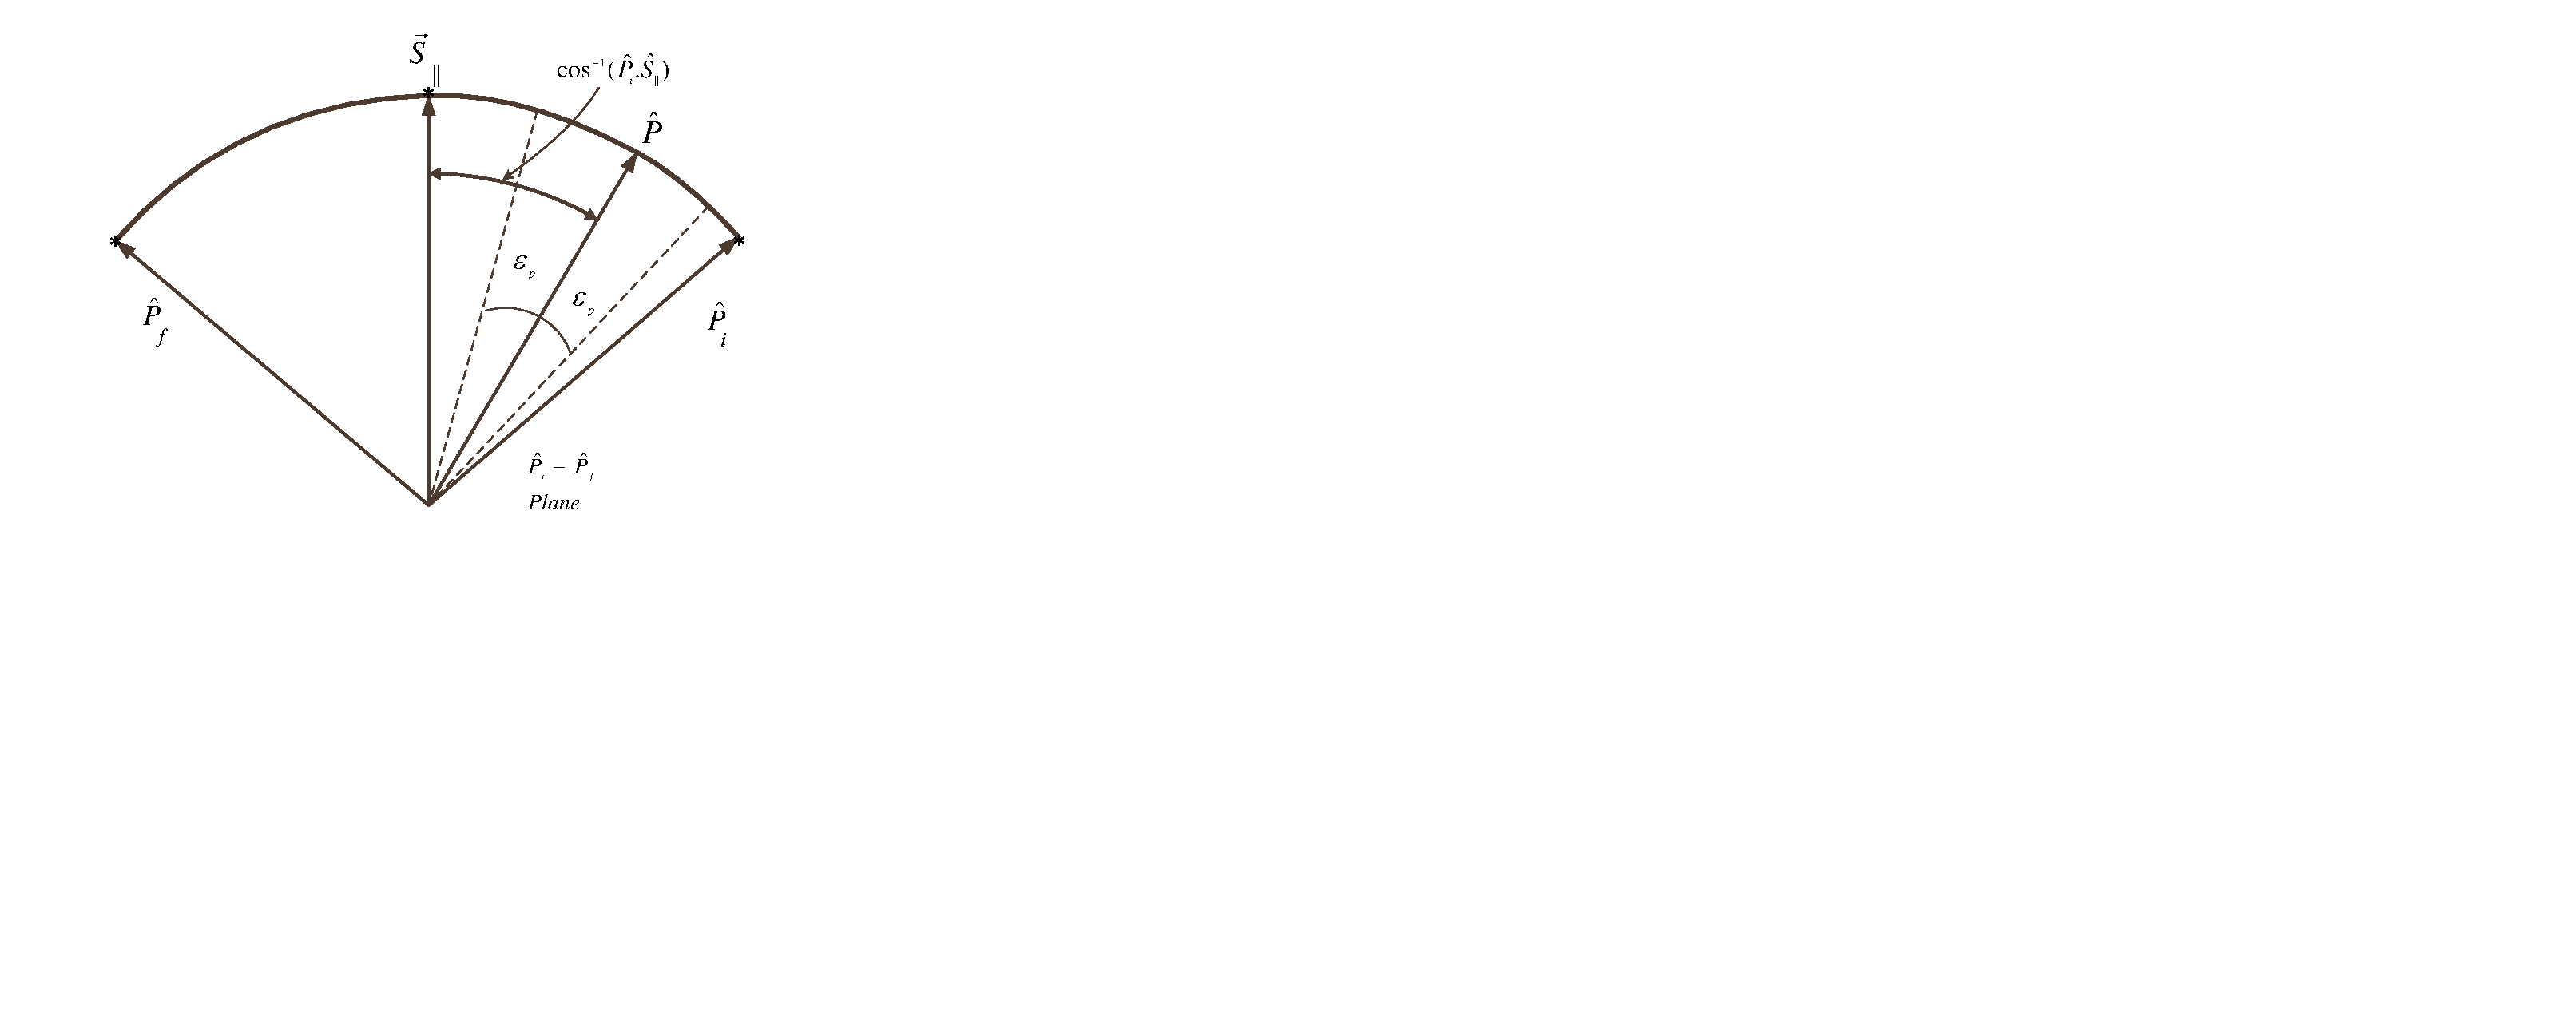
\includegraphics[width=2.3in]{./Figures/SVAS_1r}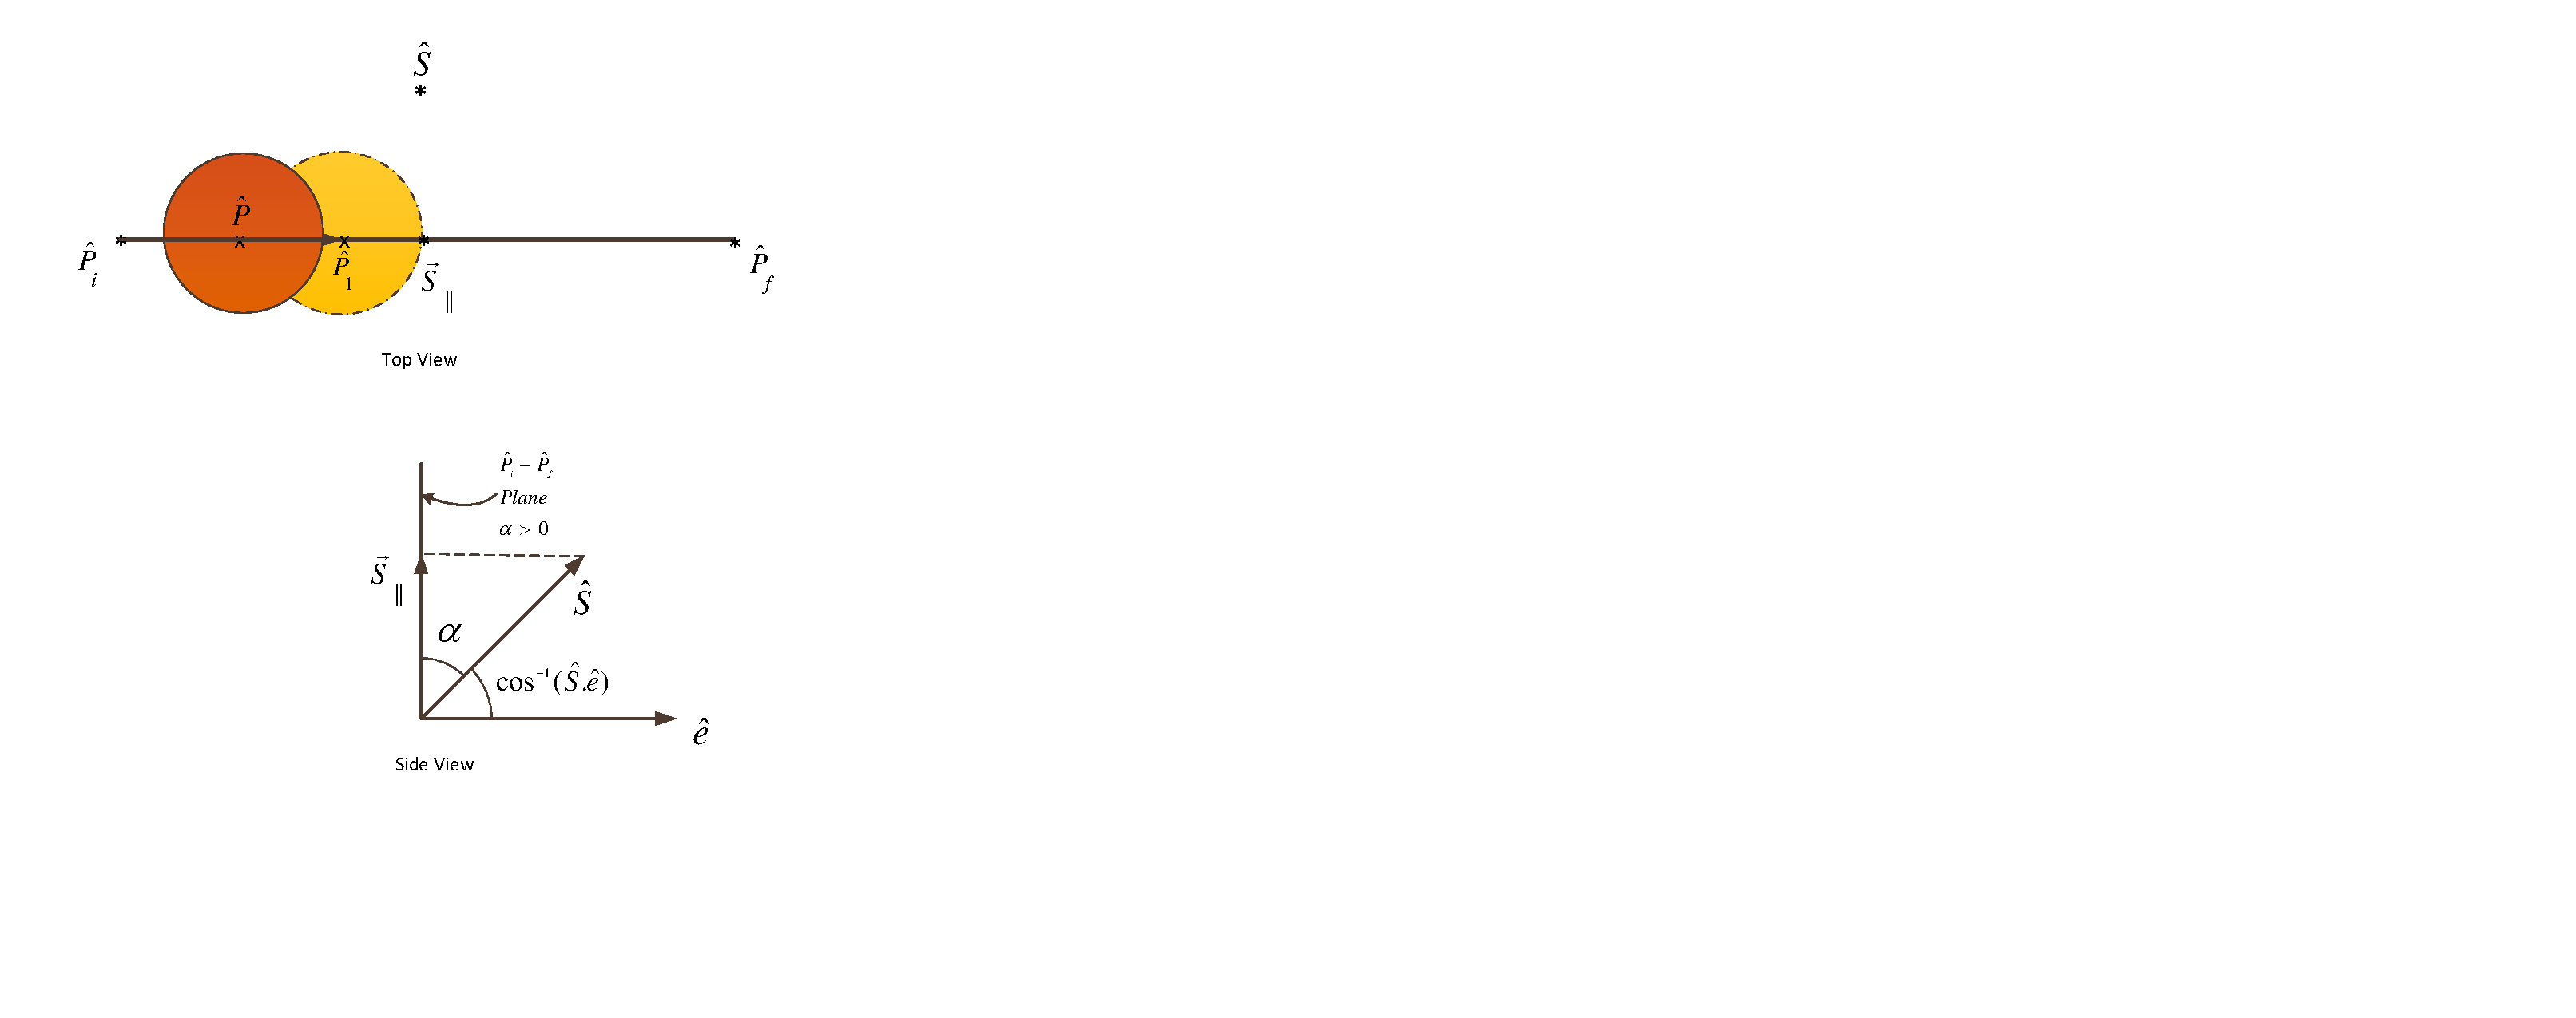
\includegraphics[width=2.3in]{./Figures/SVAS_1rb}
\end{figure}
\end{block}
\end{frame}

%-------------------------------------------------------------------------------------------------------------------------------------------------------------------
\begin{frame}
\begin{block}{Slew Maneuvers}
\begin{enumerate}[2]
\item The $2^{nd}$ slew around the unit sun vector, $\hat{S}$, via $\phi_2$.
\begin{enumerate}[a]
\item when $\alpha\neq0$
\end{enumerate}
\end{enumerate}
\begin{figure}
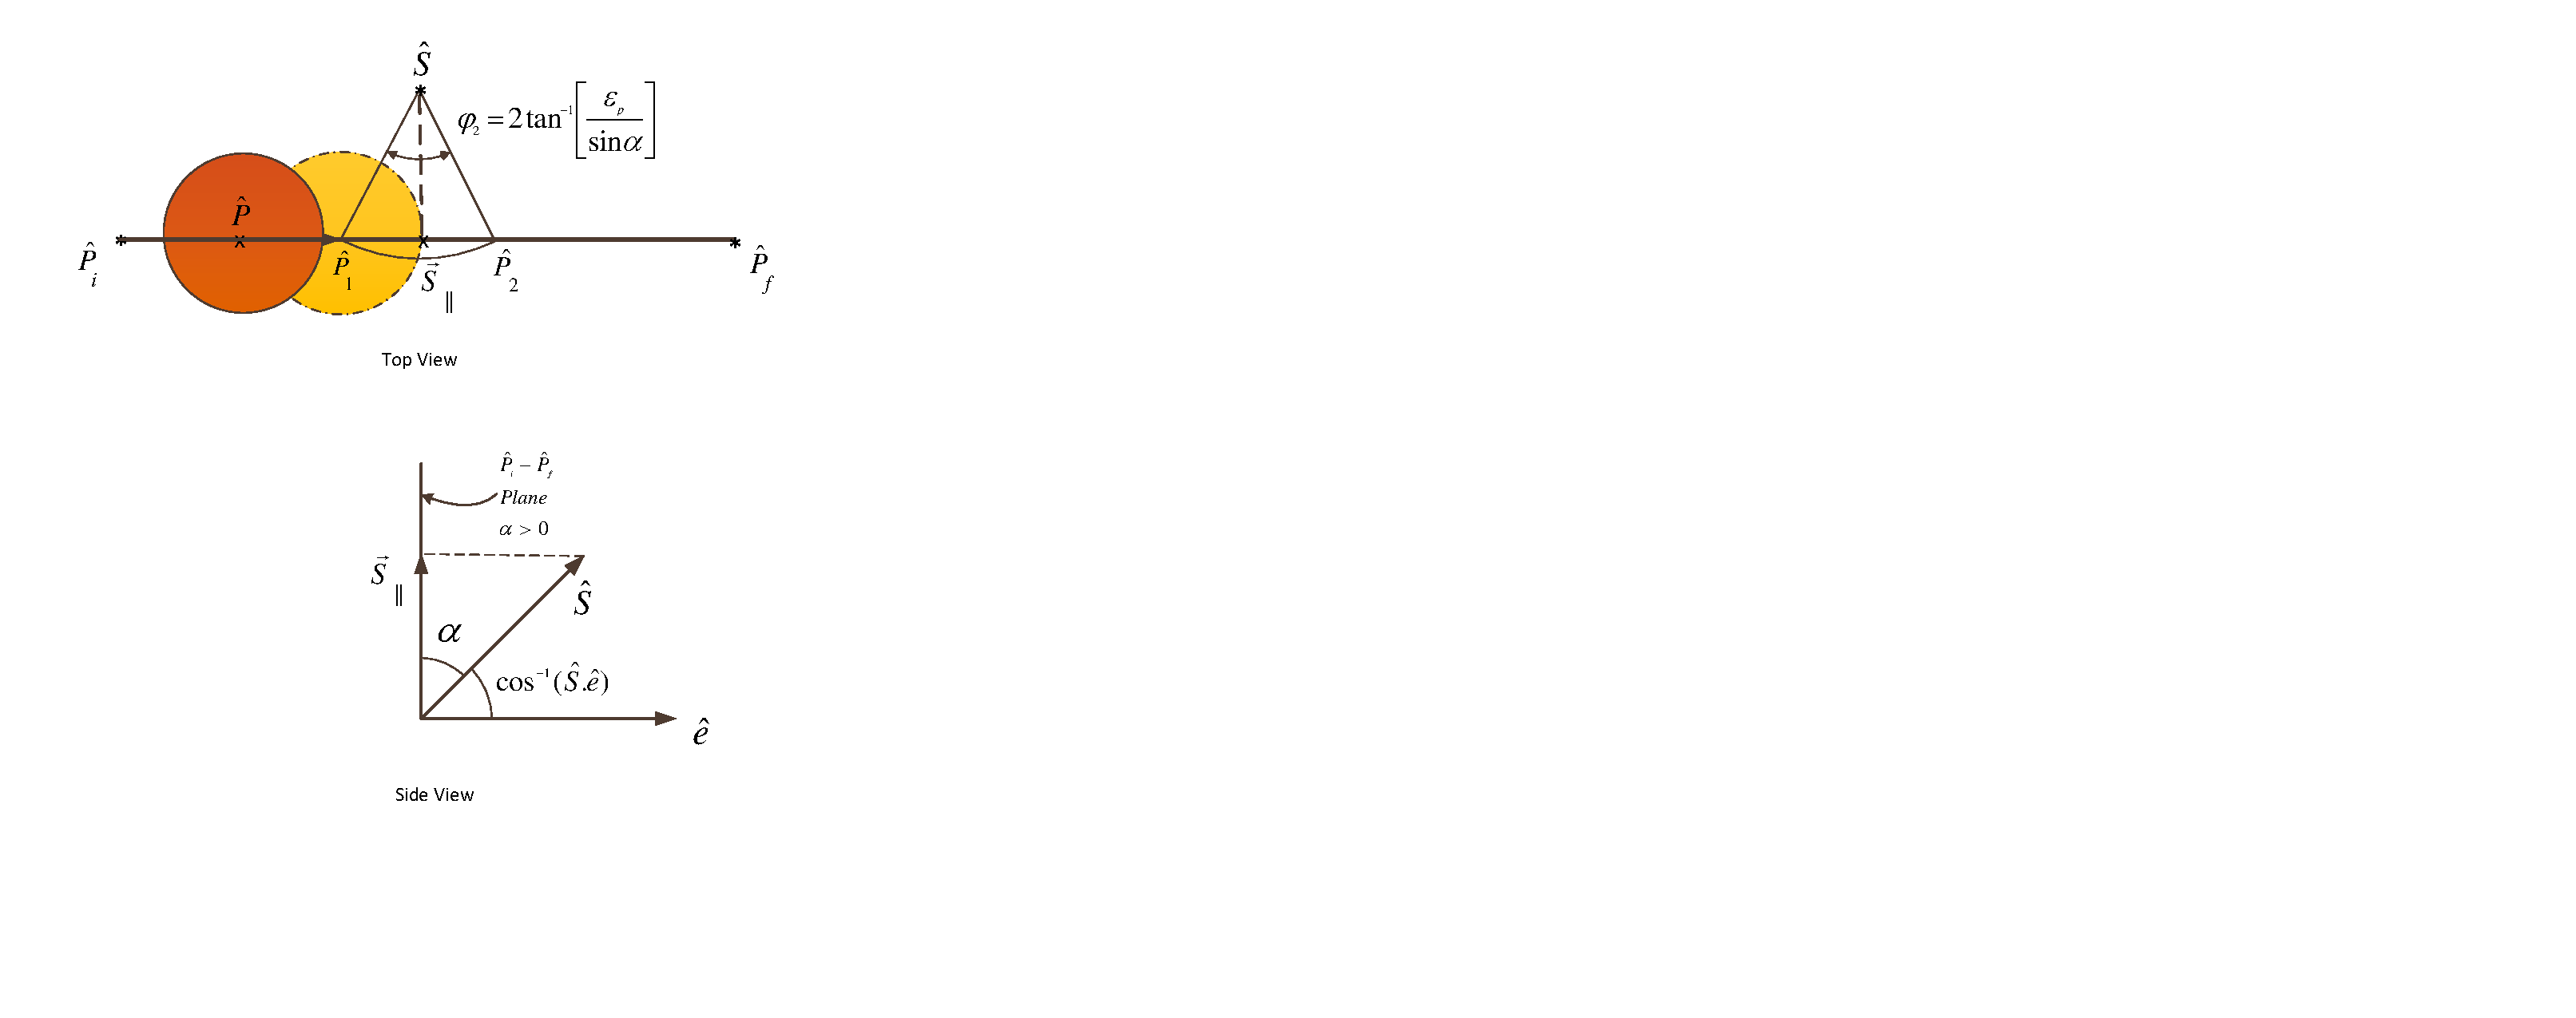
\includegraphics[width=2.3in]{./Figures/SVAS_2r}
\end{figure}
\end{block}
\end{frame}
%-------------------------------------------------------------------------------------------------------------------------------------------------------------------
\begin{frame}
\begin{block}{Slew Maneuvers}
\begin{enumerate}[2]
\item The $2^{nd}$ slew around the unit sun vector, $\hat{S}$, via $\phi_2=180^{\circ}$.
\begin{enumerate}[b)]
\item when $\alpha=0$
\end{enumerate}
\end{enumerate}
\begin{figure}
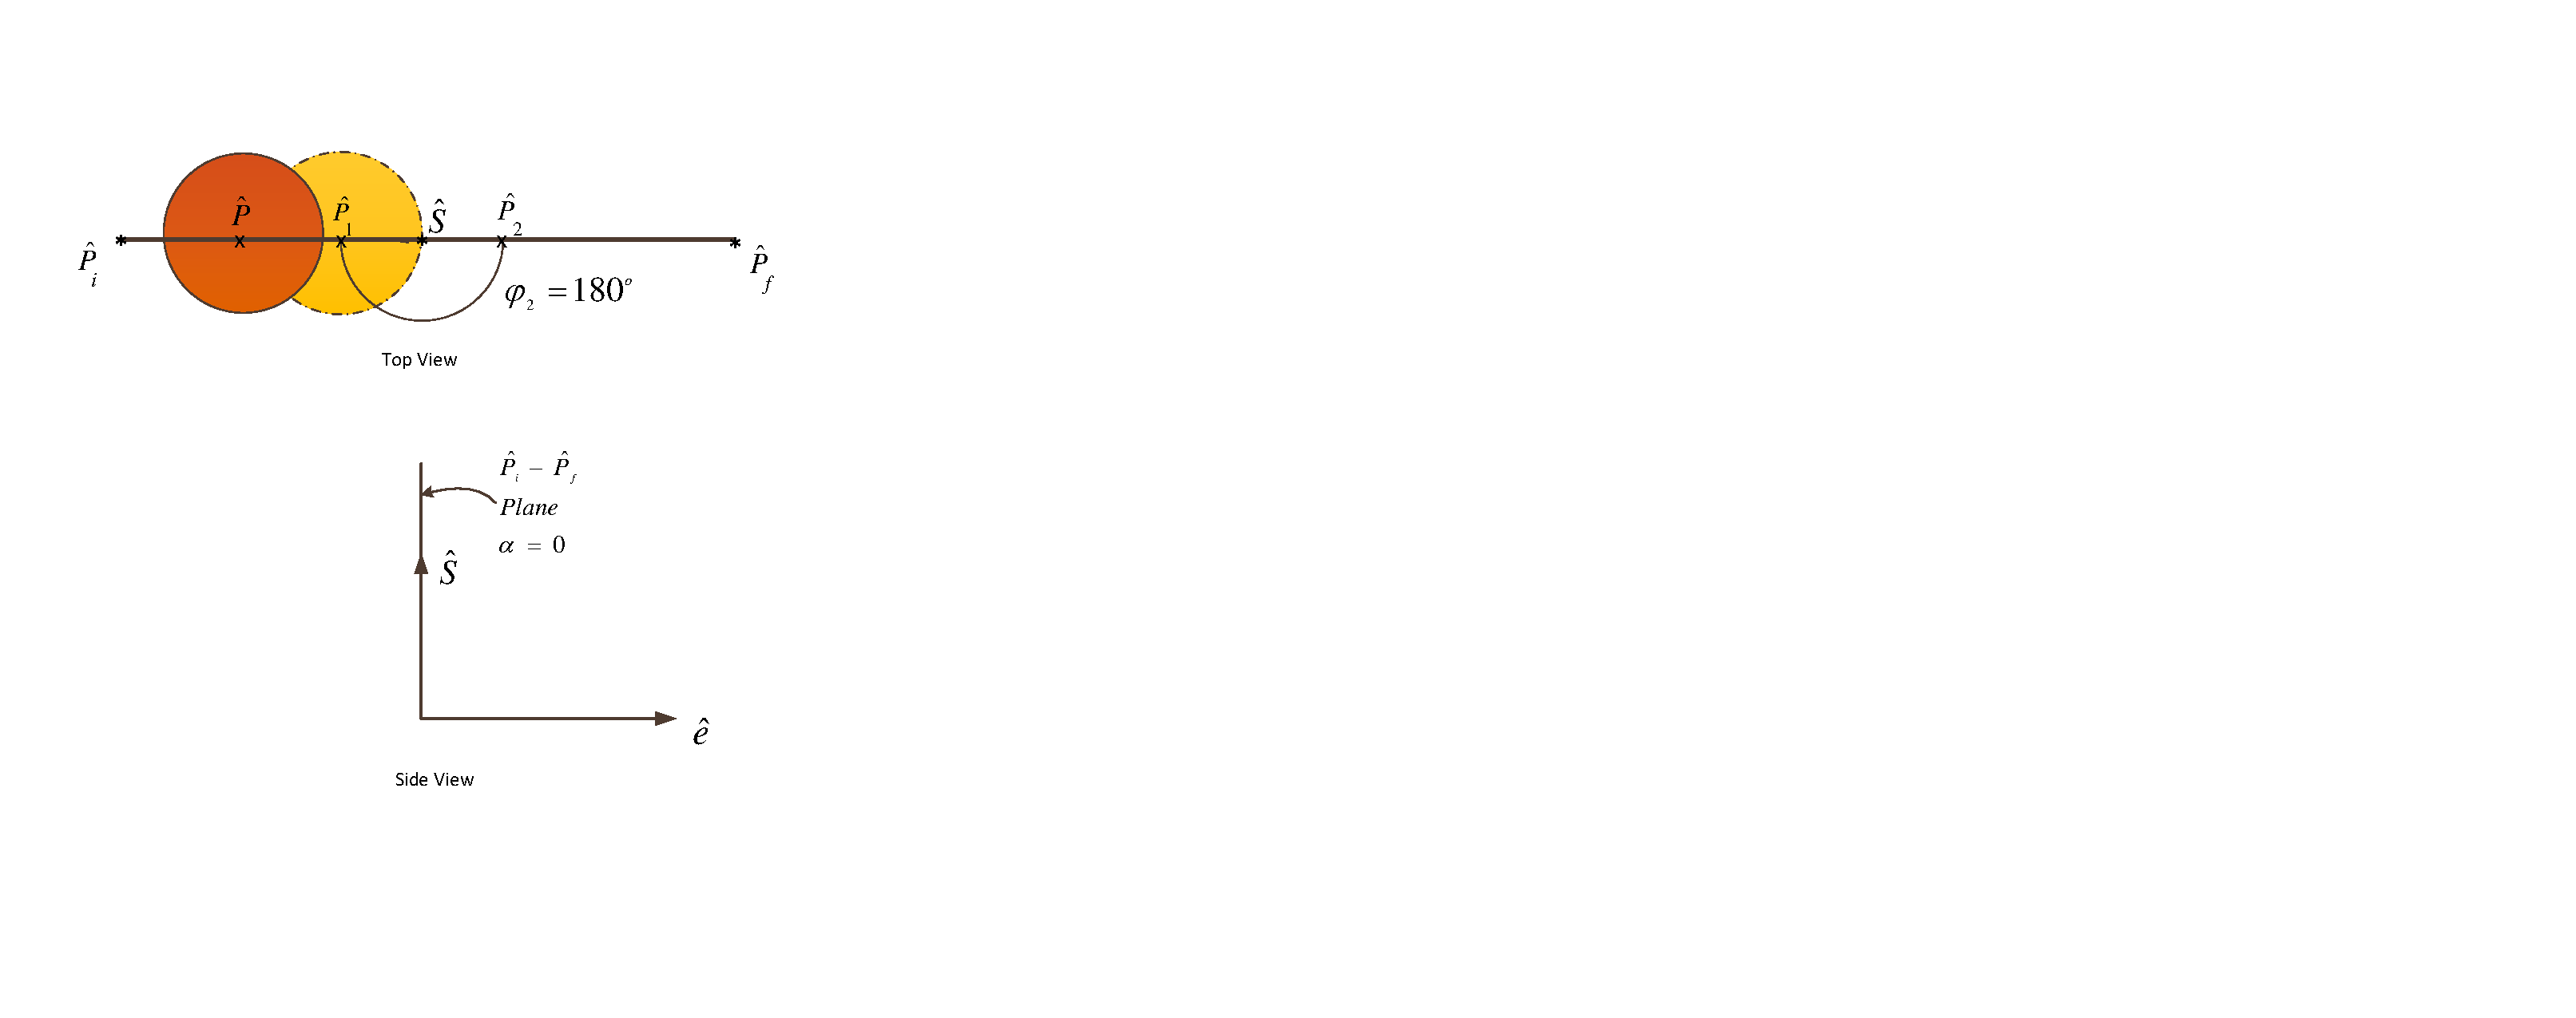
\includegraphics[width=2.3in]{./Figures/SVAS_3r}
\end{figure}
\end{block}
\end{frame}

%-------------------------------------------------------------------------------------------------------------------------------------------------------------------
\begin{frame}
\begin{block}{Slew Maneuvers}
\begin{enumerate}[3]
\item The $3^{rd}$ slew about the $\hat{e}$ through angle:
 \begin{equation}
 \phi_3=\left\{
                \begin{array}{ll}
                  \cos^{-1}(_G\hat{P}_f.\hat{P}_2)& when\  _G\hat{P}_f.\hat{P}_2\geq 0\\
                 \cos^{-1}(_G\hat{P}_f.\hat{P}_2)-2\pi& when\ _G\hat{P}_f.\hat{P}_2<0\\
                \end{array}
              \right.
 \end{equation}
\begin{figure}
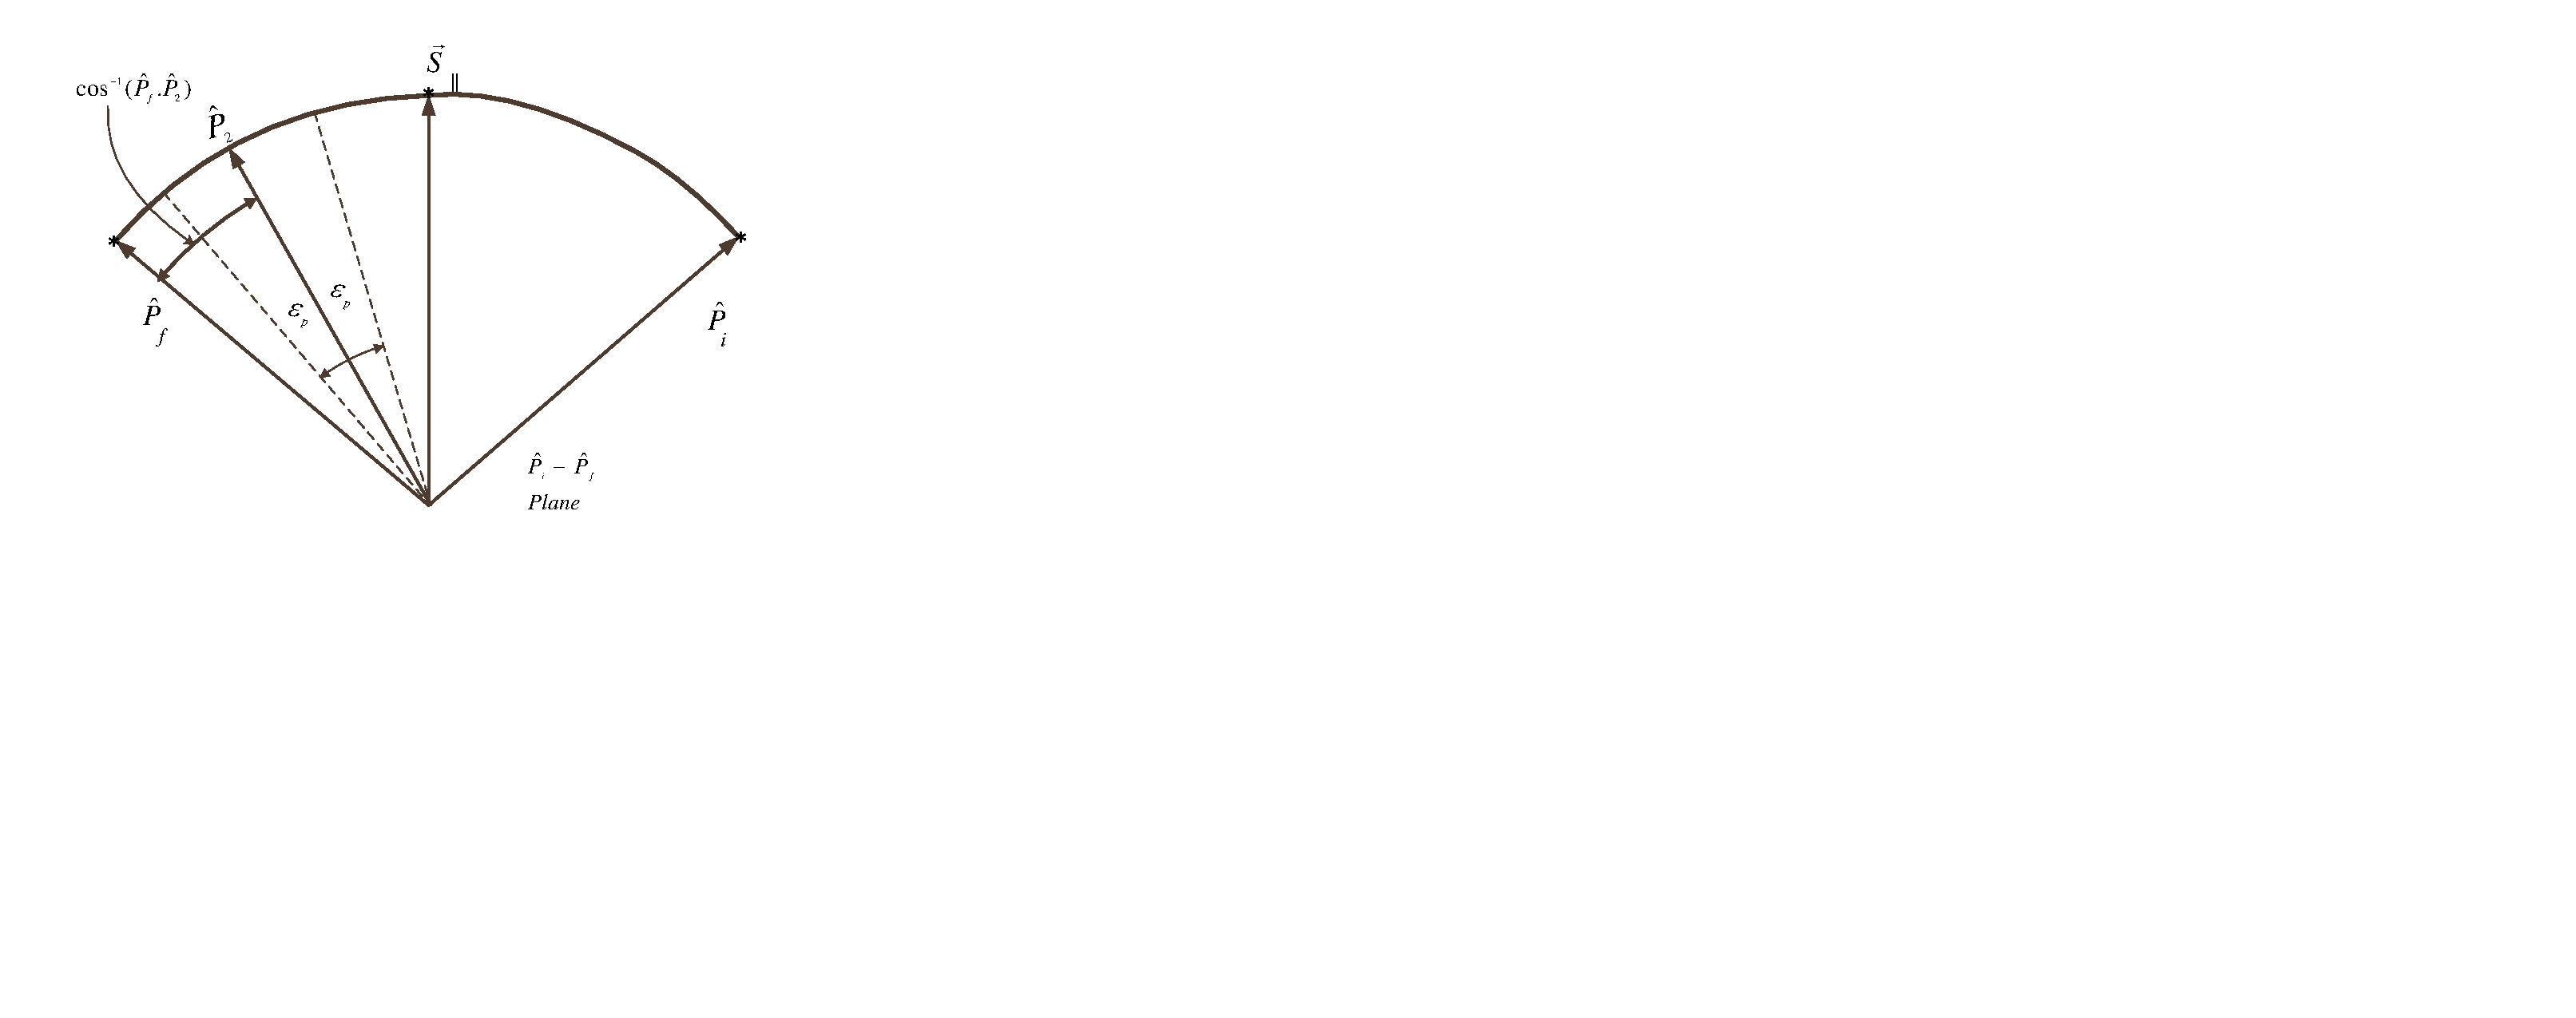
\includegraphics[width=2.3in]{./Figures/SVAS_4r}
\end{figure}
\end{enumerate}
\begin{enumerate}[4]
\item The final slew is about the instrument boresight axis to go to the final attitude. 
\end{enumerate}
\end{block}
\end{frame}


%-------------------------------------------------------------------------------------------------------------------------------------------------------------------
\begin{frame}
\begin{block}{Summary of the Algorithm}
\begin{enumerate}
\item Slew around the eigenaxis,$\hat{e}$, through angle:

 \begin{equation}\label{phi1}
 \phi_1=\left\{
                \begin{array}{ll}
                 \cos^{-1}(\hat{P}._G\hat{S}_{||})-\epsilon_p& when\  \cos^{-1}(\hat{P}._G\hat{S}_{||})-\epsilon_p\leq \pi\\
                 \cos^{-1}(\hat{P}._G\hat{S}_{||})-\epsilon_p-2\pi& when\ \cos^{-1}(\hat{P}._G\hat{S}_{||})-\epsilon_p>\pi\\
                \end{array}
              \right.
 \end{equation}
\item Slew around the $\hat{S}$ via:
 \begin{equation}\label{phi2}
 \phi_2=\left\{
                \begin{array}{ll}
                  2\tan^{-1}(\frac{\epsilon_p}{\sin\alpha})& when\  \alpha\neq 0\\
                 \pi& when\ \alpha=0\\
                \end{array}
              \right.
 \end{equation}
 \item Slew about the $\hat{e}$ through angle:
 \begin{equation}\label{phi3}
 \phi_3=\left\{
                \begin{array}{ll}
                  \cos^{-1}(_G\hat{P}_f.\hat{P}_2)& when\  _G\hat{P}_f.\hat{P}_2\geq 0\\
                 \cos^{-1}(_G\hat{P}_f.\hat{P}_2)-2\pi& when\ _G\hat{P}_f.\hat{P}_2<0\\
                \end{array}
              \right.
 \end{equation}

\item Perform the final rotation, $\phi_4$, about the instrument boresight axis to adjust the attitude. 
\end{enumerate}
\end{block}
\end{frame}

%-------------------------------------------------------------------------------------------------------------------------------------------------------------------
\begin{frame}
\begin{block}{Summary of the Algorithm}
\begin{figure}
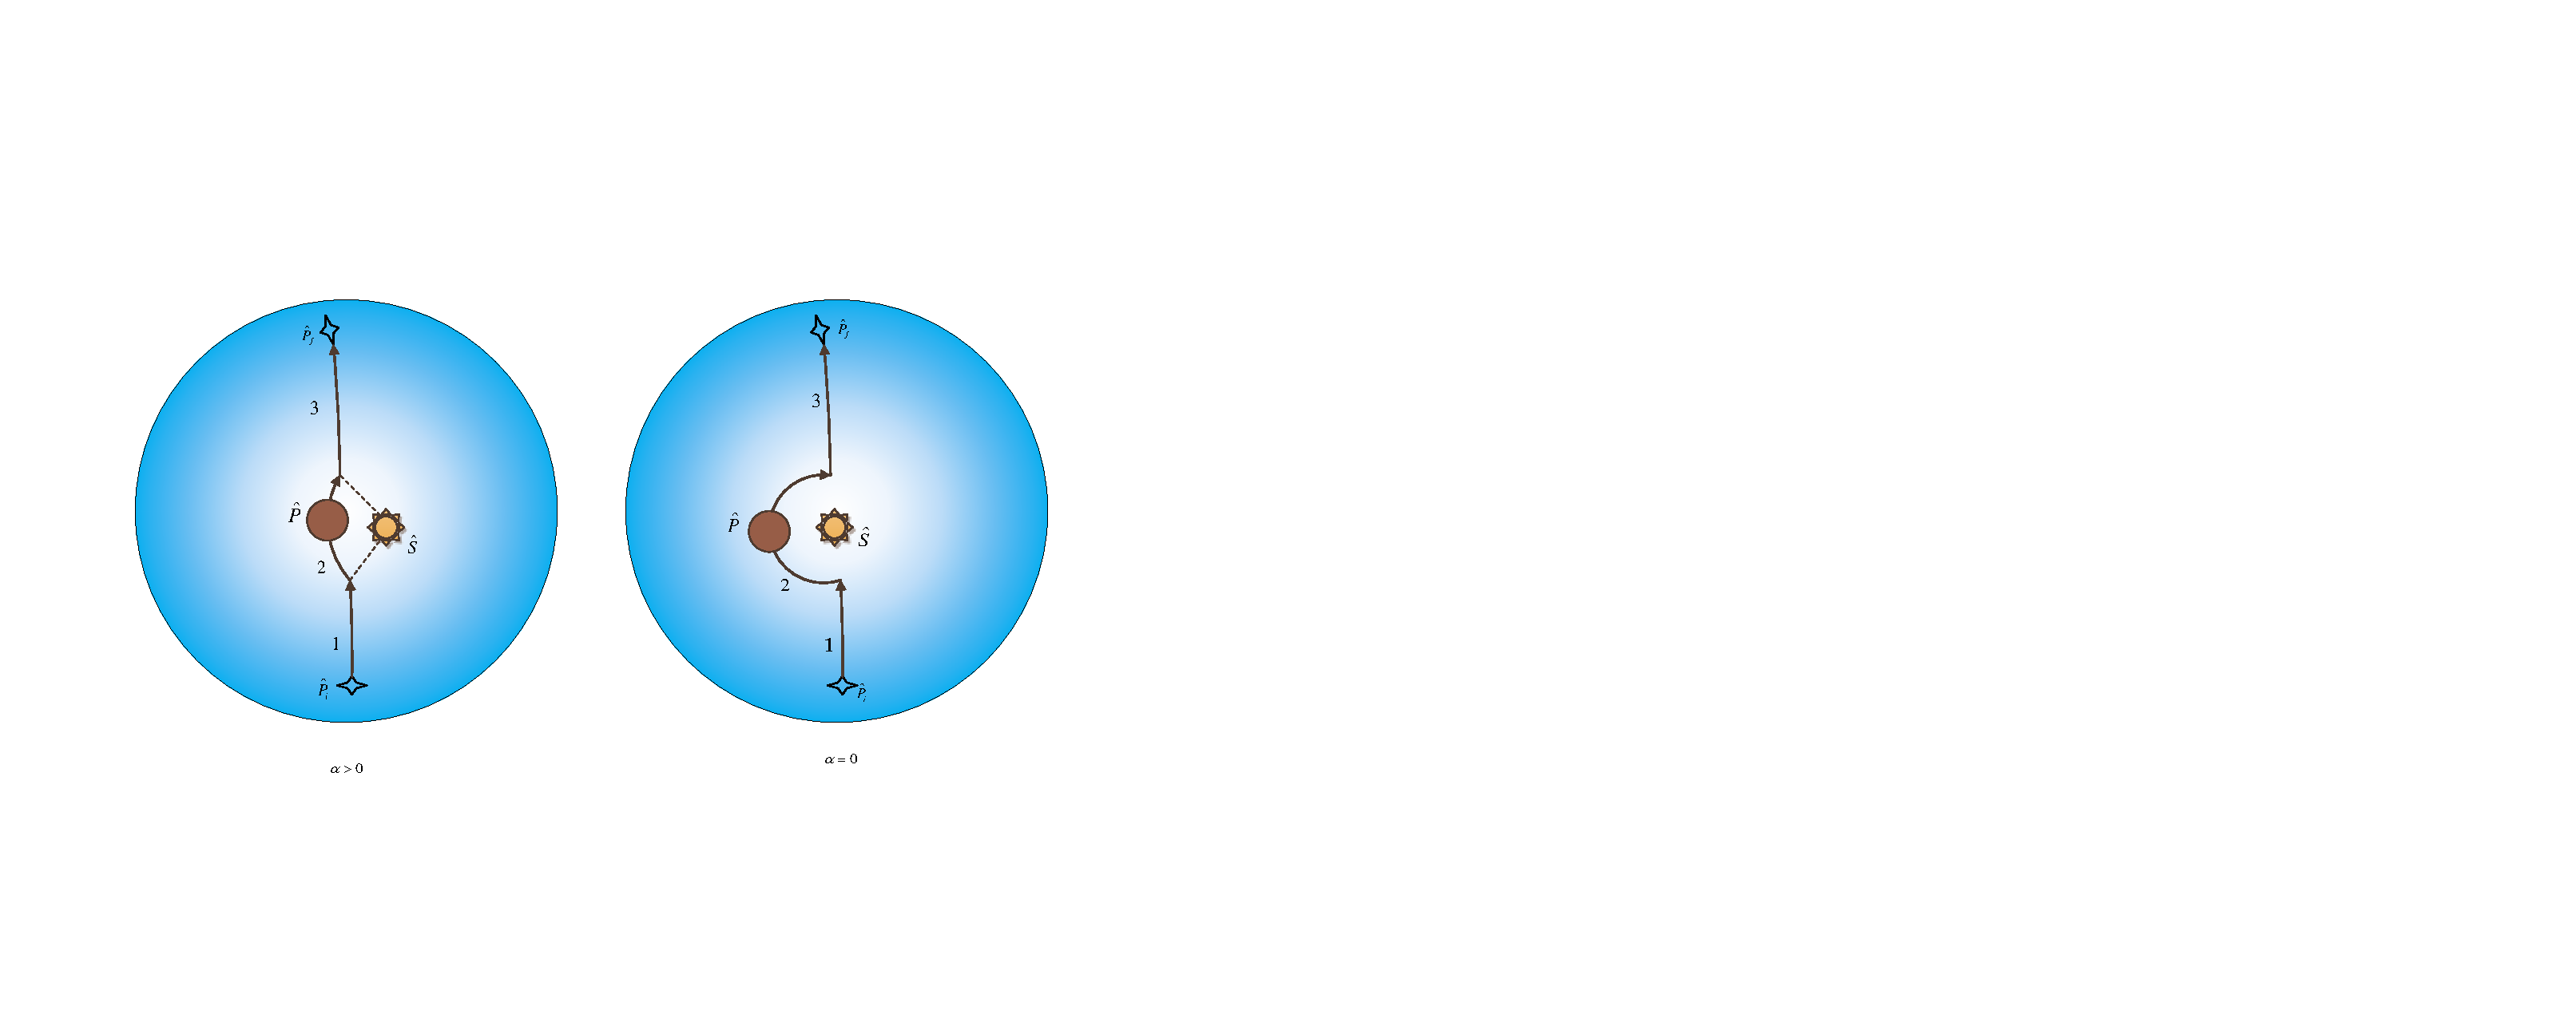
\includegraphics[width=4.85in]{./Figures/SASSchematic3}
\end{figure}
\end{block}
\end{frame}
%%-------------------------------------------------------------------------------------------------------------------------------------------------------------------
%\begin{frame}{ How we calculate the steering laws? e.g $^N\omega_c^B$}
%\begin{enumerate}
%	\item Start with the structural dynamics model
%	\begin{equation}\label{struc}
%	M\ddot{x}+ Kx=u
%	\end{equation}
%	%where $q$ is a generalized displacement vector, $M$ a mass matrix, $K$ is the stiffness matrix, and $G$ a control input distribution matrix, and $u$ a control input vector.\\
%	%Assume that:
%	%$u_{im}\leq u_i\leq u_{iM}, (i=1,2,3,4)$
%	%\item Let's write Eq.(\ref{struc}) into decoupled modal equations:
%	\item Transform Eq.(\ref{struc}) into  the modal equations:
%	\begin{equation}
%	\ddot{q}+\Omega^2 q=\phi^Tu
%	\end{equation}
%	\item Formulate a time-optimal slew maneuver in which the structural vibration is minimum.
%	\item Solve the optimal control problem. 
%	\item Use the calculated optimal control and the initial conditions (for each segment) with the S/C model to find  $^Nq_c^B$,  $^N\omega_c^B$  and  $^N\alpha_c^B$. 
%\end{enumerate}
%\end{frame}



%-------------------------------------------------------------------------------------------------------------------------------------------------------------------
\begin{frame}
\begin{block}{}
\begin{center}
{\LARGE{Computing the Steering Profiles}}
\begin{itemize}
\item Case 1)  Single-Axis, Agile Slew Maneuver with Velocity and Acceleration Constraints.
\end{itemize}
\end{center}
\end{block}
\end{frame}
%-------------------------------------------------------------------------------------------------------------------------------------------------------------------
\begin{frame}
\begin{block}{ Single-Axis, Agile Slew Maneuver with Velocity and Acceleration Constraints}

 {\bf Problem Statement:} \\ Consider the motion of a \textcolor{blue}{rigid} spacecraft around a given inertially-fixed axis, $_G\hat{e}=[e_x,e_y,e_z]^T$. The problem of minimum-time slew maneuver around the $\hat{e}$ axis can be formulated as

%\begin{columns}
\begin{minipage}{0.55\textwidth}
\begin{equation}\label{costfunction}
\underset{u}{Minimze}\ J[x(.), u(.), t_f]=\int_{t0}^{t_f} dt,
\end{equation}
subject to the following dynamic constraint
\begin{equation}\label{system}
 \Sigma:\left\{
                \begin{array}{l}
                \dot{x}_1=x_2, \\
                \dot{x}_2=M/I_{\hat{e}}^{G/G*}=u, \\
                \end{array}
              \right.
 \end{equation}
where $x_1\triangleq\phi$ and $x_2=\dot{\phi}$. 
\end{minipage}
\begin{minipage}{0.35\textwidth}
\begin{center}
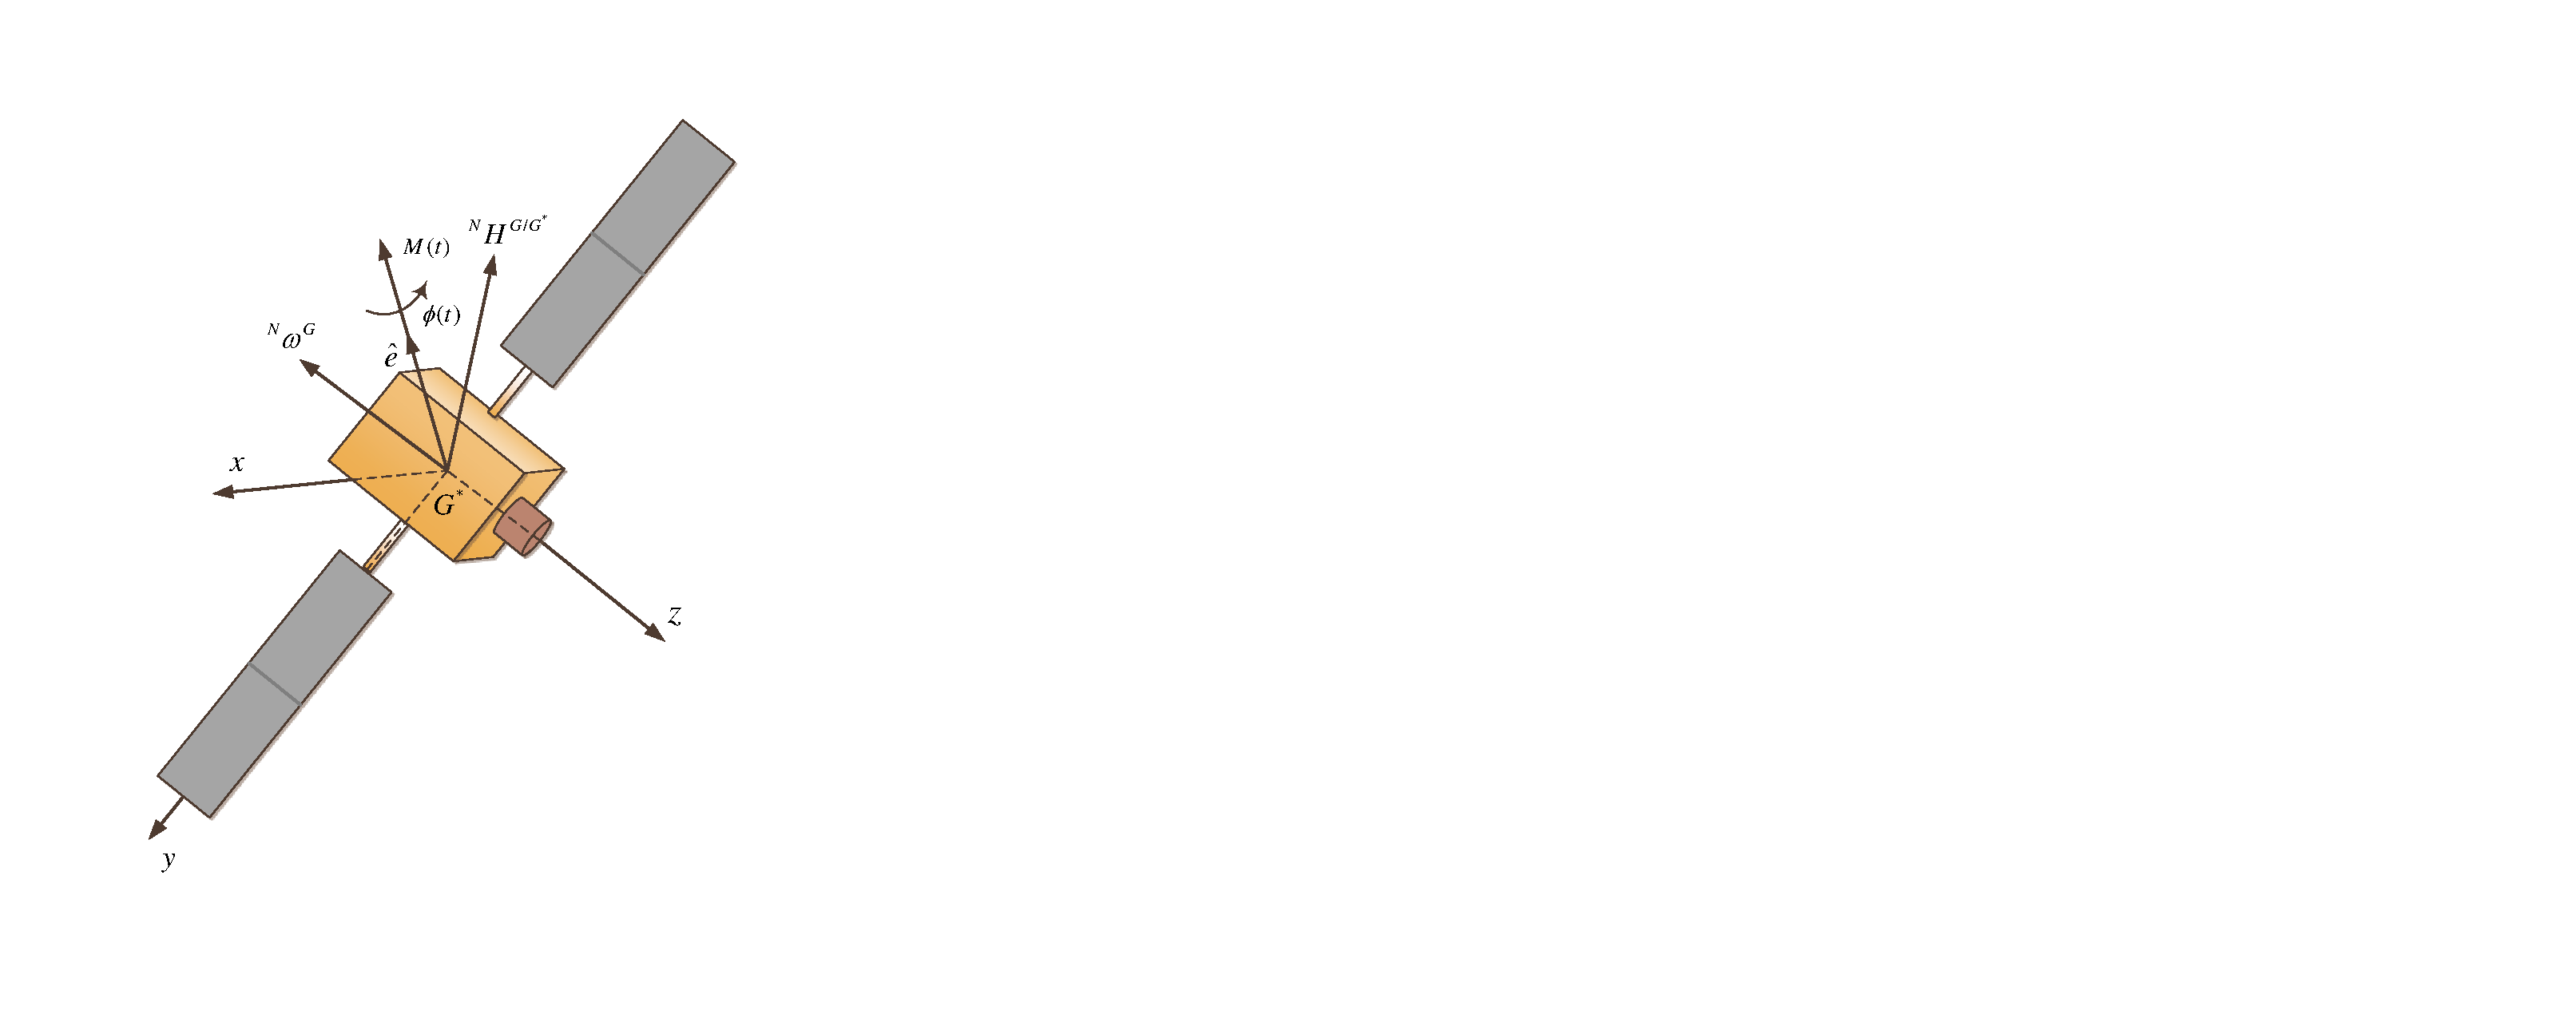
\includegraphics[width=2.25in]{./Figures/Spacecraft}      
\end{center}
\end{minipage}
%\end{columns}
\end{block}
\end{frame}
%-------------------------------------------------------------------------------------------------------------------------------------------------------------------
\begin{frame}
\begin{block}{ Single-Axis, Agile Slew Maneuver with Velocity and Acceleration Constraints}
The boundary conditions are
\begin{equation}\label{Bcs}
 BCs:\left\{
                \begin{array}{l}
                \phi(t_0)=0, \phi(t_f)=\phi_{f},\\
               \dot{\phi}(t_0)=\dot{\phi}_{0},\dot{ \phi}(t_f)=\dot{\phi}_{f}, \\
                \end{array}
              \right.
 \end{equation}
and velocity (state) and acceleration (control) constraints are

\begin{equation}\label{constraints1}
 C_1:\left\{
                \begin{array}{l}
               |x_2=\dot{\phi}|\leq \dot{\phi}_{max},\\
              |u=\ddot{\phi}|\leq \ddot{\phi}_{max},\\
                \end{array}
              \right.
 \end{equation}
in which
\begin{equation}
\dot{\phi}_{max}=[I^{w/w^*}]^{-1}[^NH^{G/G*}-(I^{G/G*}+I^{w/w*})^N\omega^G]/(e_x+e_y+e_z),
\end{equation}


%\end{minipage}
%\begin{minipage}{0.35\textwidth}
%\begin{center}
%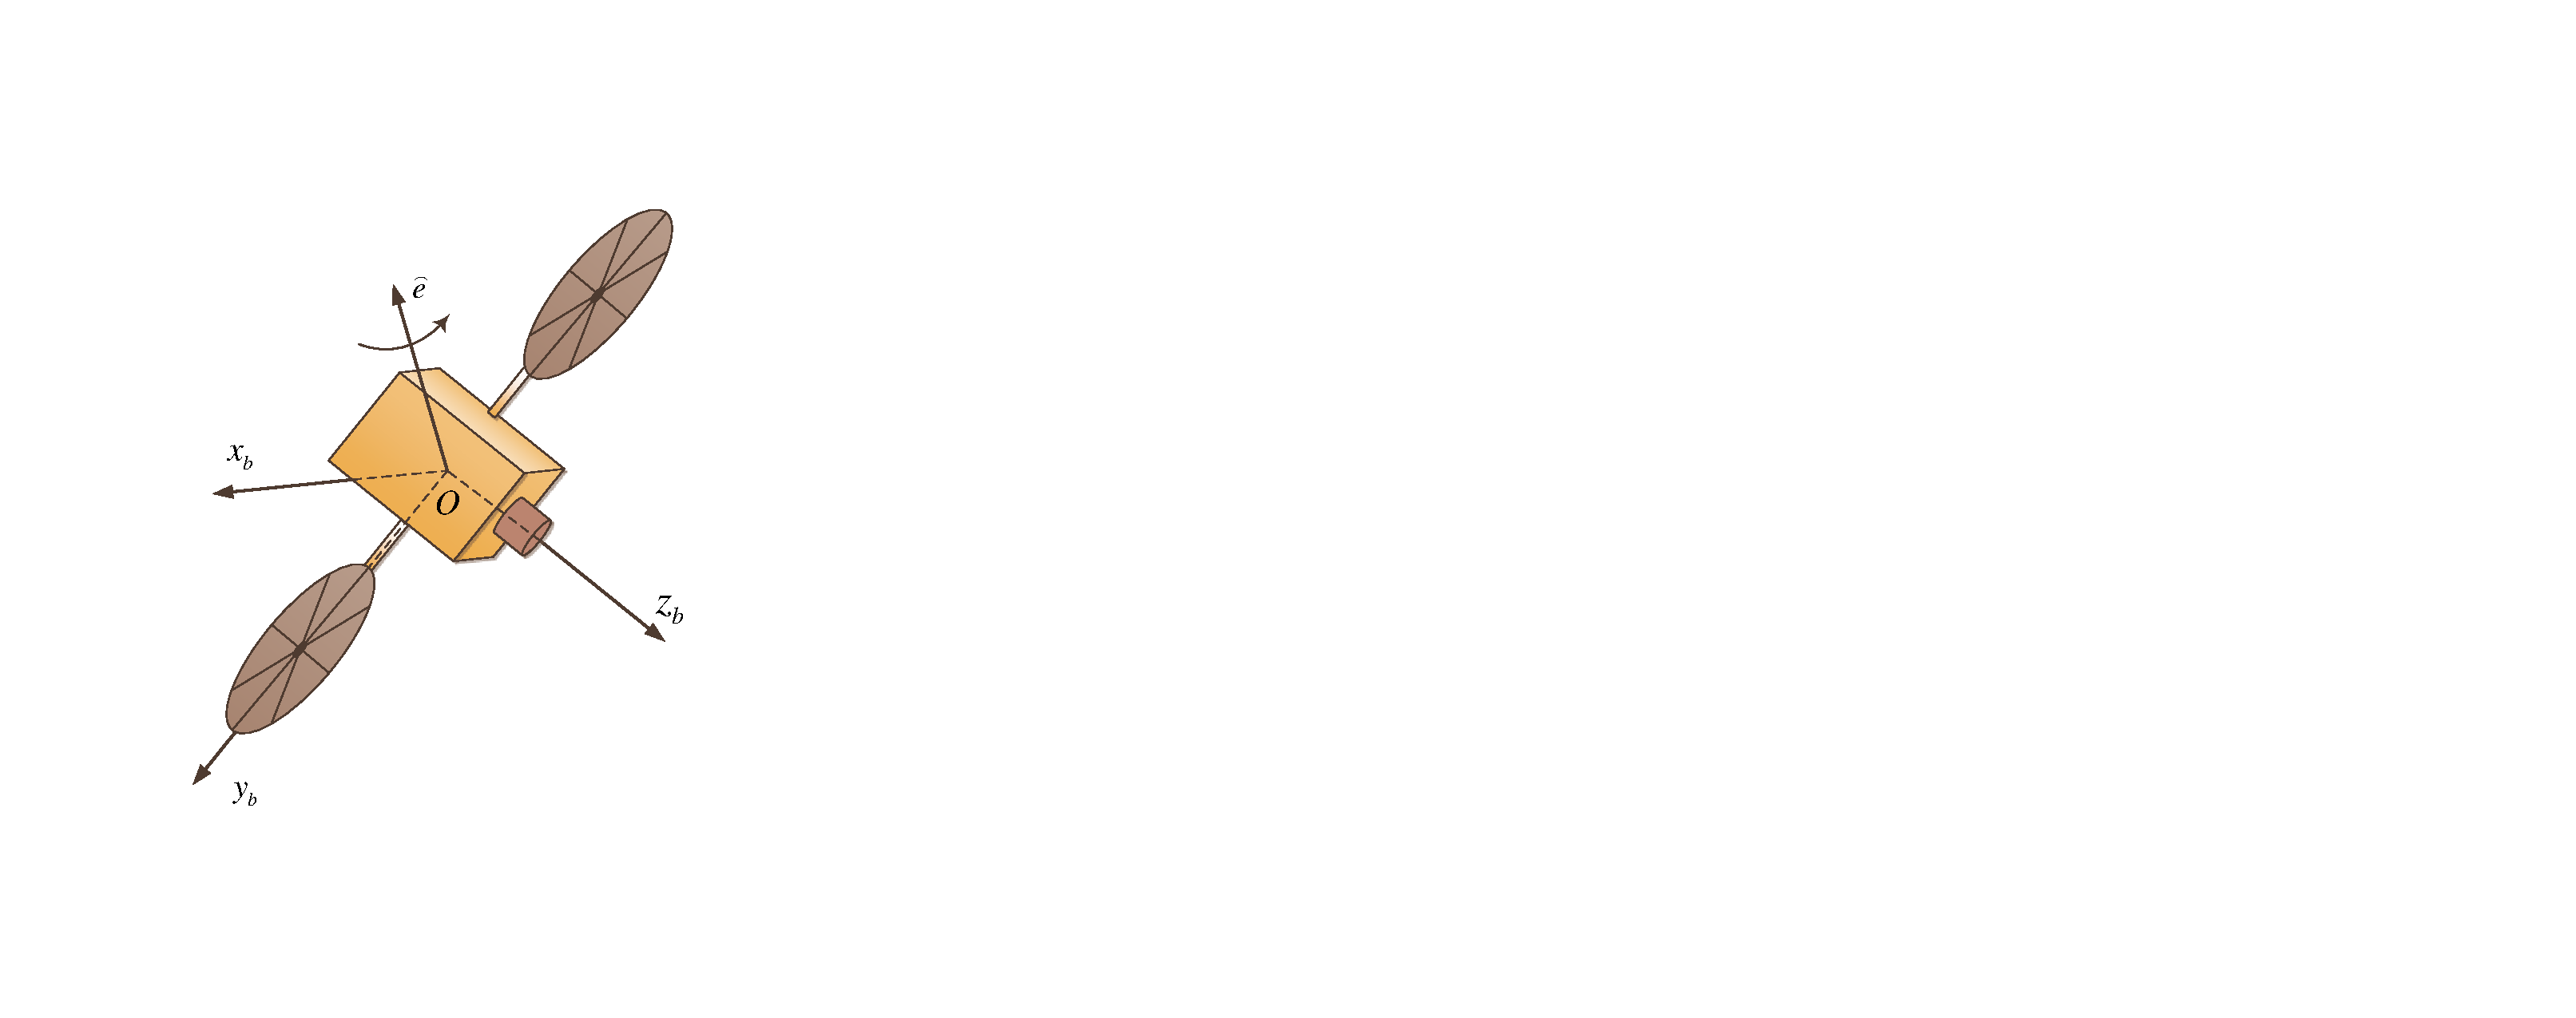
\includegraphics[width=2in]{./Spacecraft3}      
%\end{center}
%\end{minipage}
%\end{columns}
\end{block}
\end{frame}
%-------------------------------------------------------------------------------------------------------------------------------------------------------------------
\begin{frame}
\begin{block}{ Single-Axis, Agile Slew Maneuver with Velocity and Acceleration Constraints}
 and
 \begin{equation}\label{phiddotmax}
\ddot{\phi}_{max}=_B\hat{e}^T\  _BM_{max}/I_{\hat{e}}^{G/G*},
\end{equation}
where $^NH^{G/G*}$ is the total angular momentum of the gyrostat with respect to its center of mass, $G^*$, in the $N$-frame. $I^{G/G^*}$ and $I^{w/w*}$ represent the inertia dyadic of the gyrostat and reaction wheel with respect to their center of masses, respectively. $_BM_{max}$ is the maximum generated torque along the body-axes in the body frame.\\
%Find the optimal steering laws: $^Bq^R$, $^B\omega^R$, and $^B\alpha^R$.
\vspace{0.5in}

{\bf Find:} $\phi(t)$, $\dot{\phi}(t)$, and $\ddot{\phi}(t)$.
%\end{minipage}
%\begin{minipage}{0.35\textwidth}
%\begin{center}
%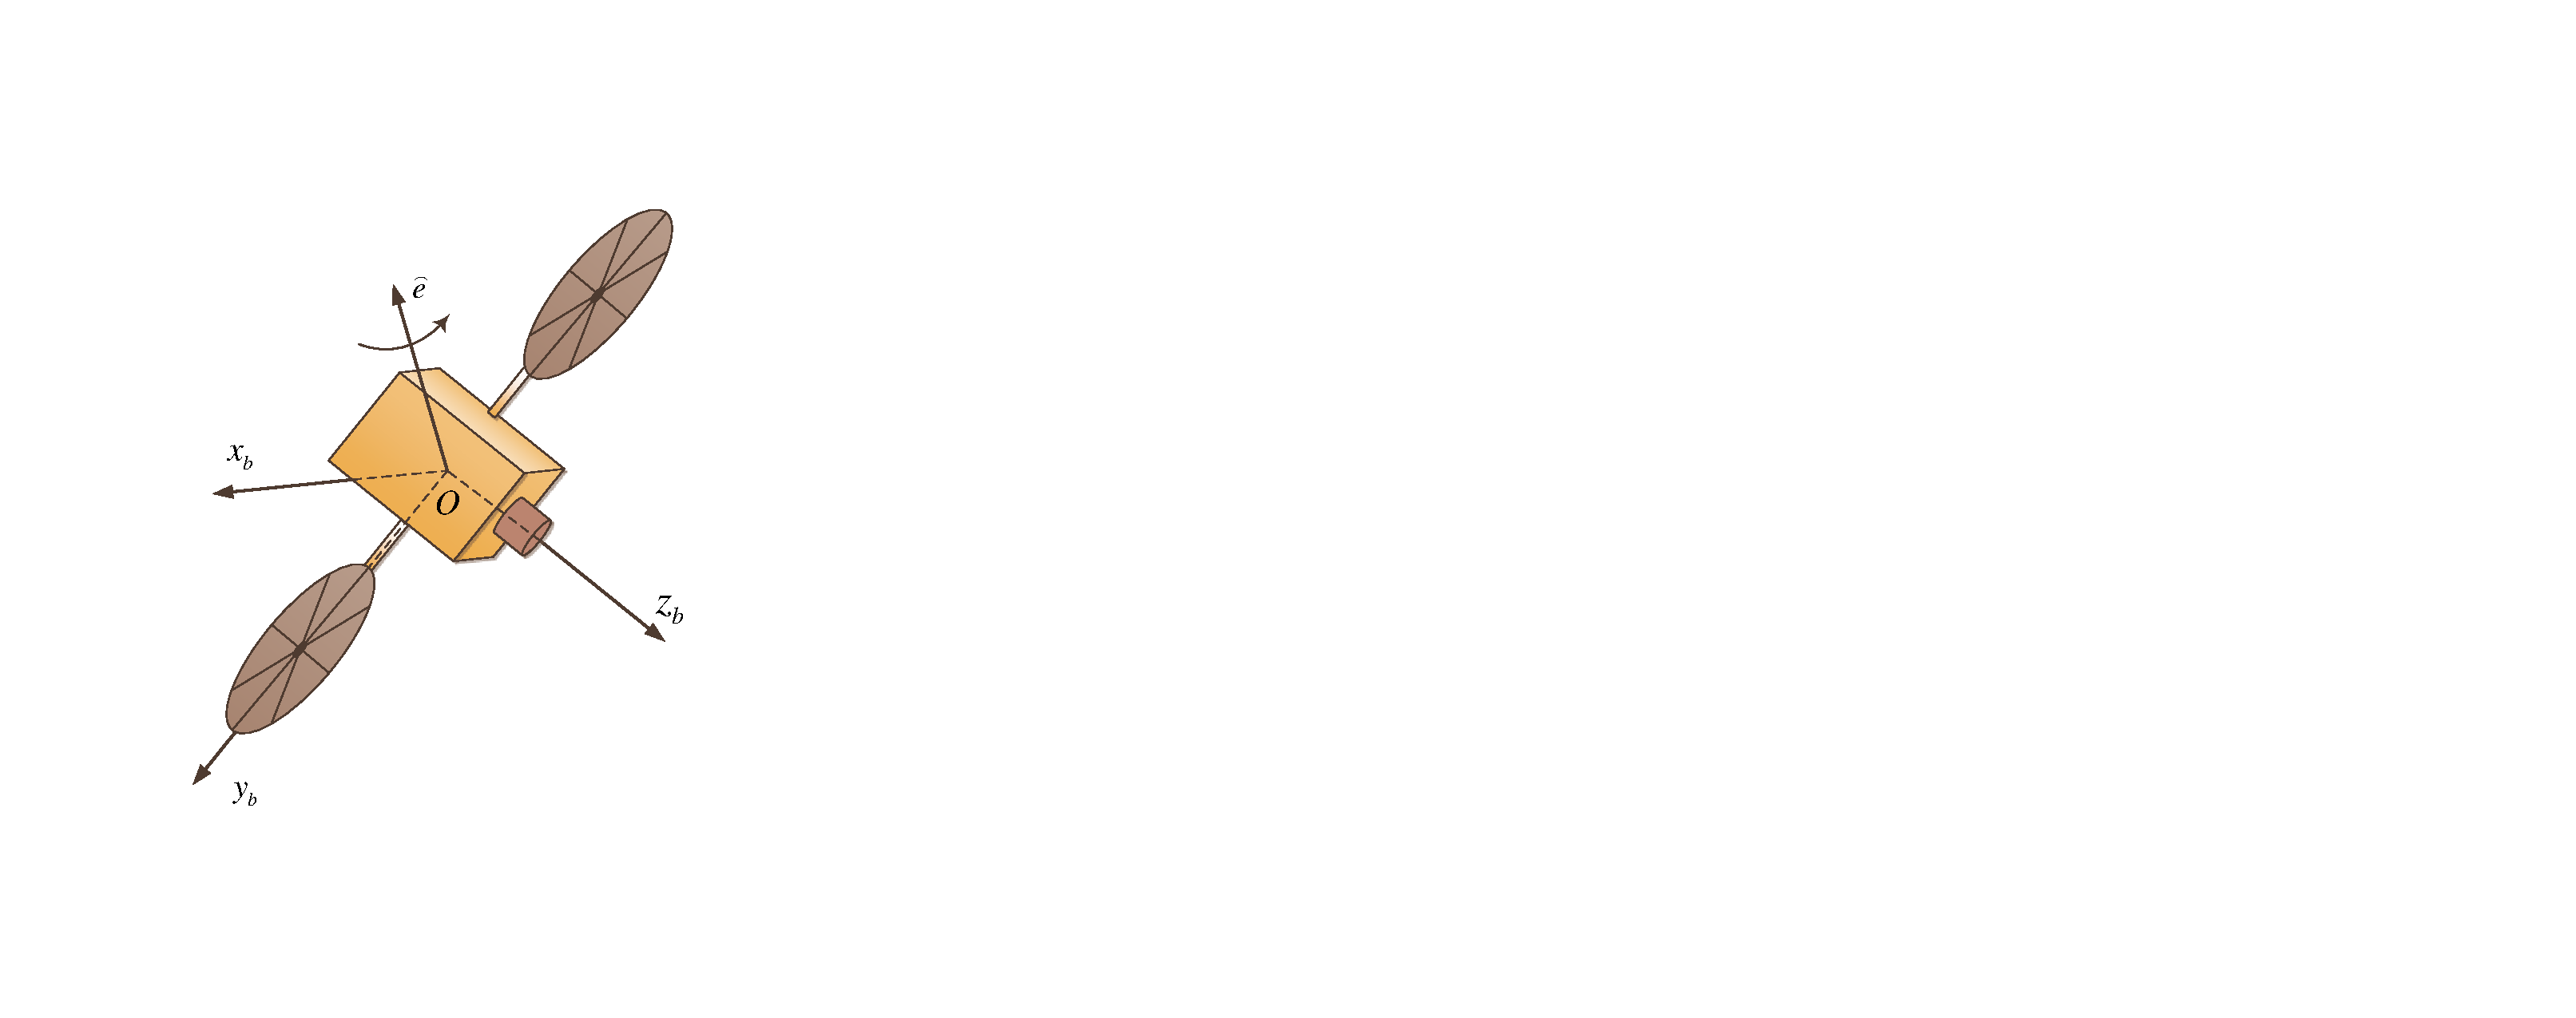
\includegraphics[width=2in]{./Spacecraft3}      
%\end{center}
%\end{minipage}
%\end{columns}
\end{block}
\end{frame}


%-------------------------------------------------------------------------------------------------------------------------------------------------------------------
\begin{frame}
\begin{block}{ Single-Axis, Agile Slew Maneuver with Velocity and Acceleration Constraints}
\small{
Using the Pontryagin's minimum principle (PMP), we derive the necessary conditions for the optimal solution as follows:
\begin{enumerate}
\item State Eqs.:
\begin{equation}
\left\{
                \begin{array}{l}
                \dot{x}_1=x_2, \\
                \dot{x}_2=u, \\
                \dot{x}_3=(x_2+\dot{\phi}_{max})^2\mathbb{U}(-x_2-\dot{\phi}_{max})+(\dot{\phi}_{max}-x_2)^2\mathbb{U}(x_2-\dot{\phi}_{max}),
                \end{array}
              \right.
\end{equation}
where the unit step function, $\mathbb{U}$, is defined as
\begin{equation}
\mathbb{U}(X)=\left\{
                \begin{array}{lI}
           1,&X> 0,\\
           0,& X\leq 0.
                \end{array}
              \right.
 \end{equation}
Note:  ($x_3(t_0)=x_3(t_f)=0$ \& $x_3(t)\geq 0$ ) $\rightarrow x_3(t)=0, \foral t\in[t_0, t_f]. $  
\item Hamlitonian:
\begin{equation}
\begin{split}
\mathscr{H}=& 1+\lambda_1x_2+\lambda_2 u+\lambda_3\Big[(x_2+\dot{\phi}_{max})^2\mathbb{U}(-x_2-\dot{\phi}_{max})\\
& (\dot{\phi}_{max}-x_2)^2\mathbb{U}(x_2-\dot{\phi}_{max})\Big]
\end{split}
\end{equation}
\end{enumerate}
}
\seti
\end{block}
\end{frame}

%-------------------------------------------------------------------------------------------------------------------------------------------------------------------
\begin{frame}
\begin{block}{ Single-Axis, Agile Slew Maneuver with Velocity and Acceleration Constraints}
\begin{enumerate}
\conti
\small{
\item Costate Eqs.:
\begin{equation}
\left\{\begin{array}{l}
               \dot{\lambda}_1=-\frac{\partial{\mathscr{H}}}{\partial{x_1}}=0,\\
               \dot{\lambda}_2=-\frac{\partial{\mathscr{H}}}{\partial{x_2}}=-\lambda_1-2\lambda_3(x_2+\dot{\phi}_{max})\mathbb{U}(-x_2-\dot{\phi}_{max})\\
+2\lambda_3(\dot{\phi}_{max}-x_2)\mathbb{U}(x_2-\dot{\phi}_{max}),\\
              \dot{\lambda}_3=-\frac{\partial{\mathscr{H}}}{\partial{x_3}}=0.\\
                \end{array}
              \right.
\end{equation}
\item Applying the Pontryagin's minimum principle (PMP),
\begin{equation}
u^*=arg \underset{u\in\mathcal{U}}{min} \mathscr{H},
\end{equation}
where $\mathcal{U}$ defines the domain of feasible controls. The optimal control can be determined as
\begin{equation}
u^*(t)=\left\{
                \begin{array}{lI}
           \ddot{\phi}_{max}&\lambda_2<0,\\
           ?& \lambda_2=0,\\
           -\ddot{\phi}_{max}&\lambda_2>0.
                \end{array}
              \right.
\end{equation}
 }
\end{enumerate}
\seti
This is a {\it singular arc} optimal control problem.
\end{block}
\end{frame}

%-------------------------------------------------------------------------------------------------------------------------------------------------------------------
\begin{frame}
\begin{block}{ Single-Axis, Agile Slew Maneuver with Velocity and Acceleration Constraints}
\begin{enumerate}
\conti
\item Determining the optimal control in the singular arc:
\begin{equation}
\frac{d^2}{dt^2}\Big(\frac{\partial \mathscr{H}}{\partial u}\Big)=\ddot{\lambda}_2=0\rightarrow \dot{x}_2=0\rightarrow u^*=0
\end{equation}
\item Checking the Generalized Legendre-Clebsch condition for optimality:
\begin{equation}
(-1)^2\frac{\partial}{\partial u}\Big[\frac{d^2}{dt^2}\Big(\frac{\partial \mathscr{H}}{\partial u}\Big)\Big]=1\geq 0
\end{equation}
\item The transversality condition:
\begin{equation}
\mathscr{H}|_{(*,t_f)}=0\  \text{and} \ \mathscr{H}\neq\mathscr{H}(t)\rightarrow \mathscr{H}=0, \forall t\in[t_0, t_f].
\end{equation}
\end{enumerate}
\seti
\end{block}
\end{frame}
%-------------------------------------------------------------------------------------------------------------------------------------------------------------------
\begin{frame}
\begin{block}{ Single-Axis, Agile Slew Maneuver with Velocity and Acceleration Constraints}
\small{
\begin{itemize}
\item Angular acceleration profile (bang-off-bang):
\end{itemize}
 \begin{equation}\label{phidd_cons}
 \ddot{\phi}(t)=u=\left\{
                \begin{array}{ll}
                \ddot{\phi}_{max}& when\  t_0\leq t\leq t_1,\\
                 0& when\  t_1\leq t \leq t_2,\\
                 -\ddot{\phi}_{max}& when \ t_2\leq t\leq t_f.
                \end{array}
              \right.
\begin{minipage}{0.35\textwidth}
\begin{center}
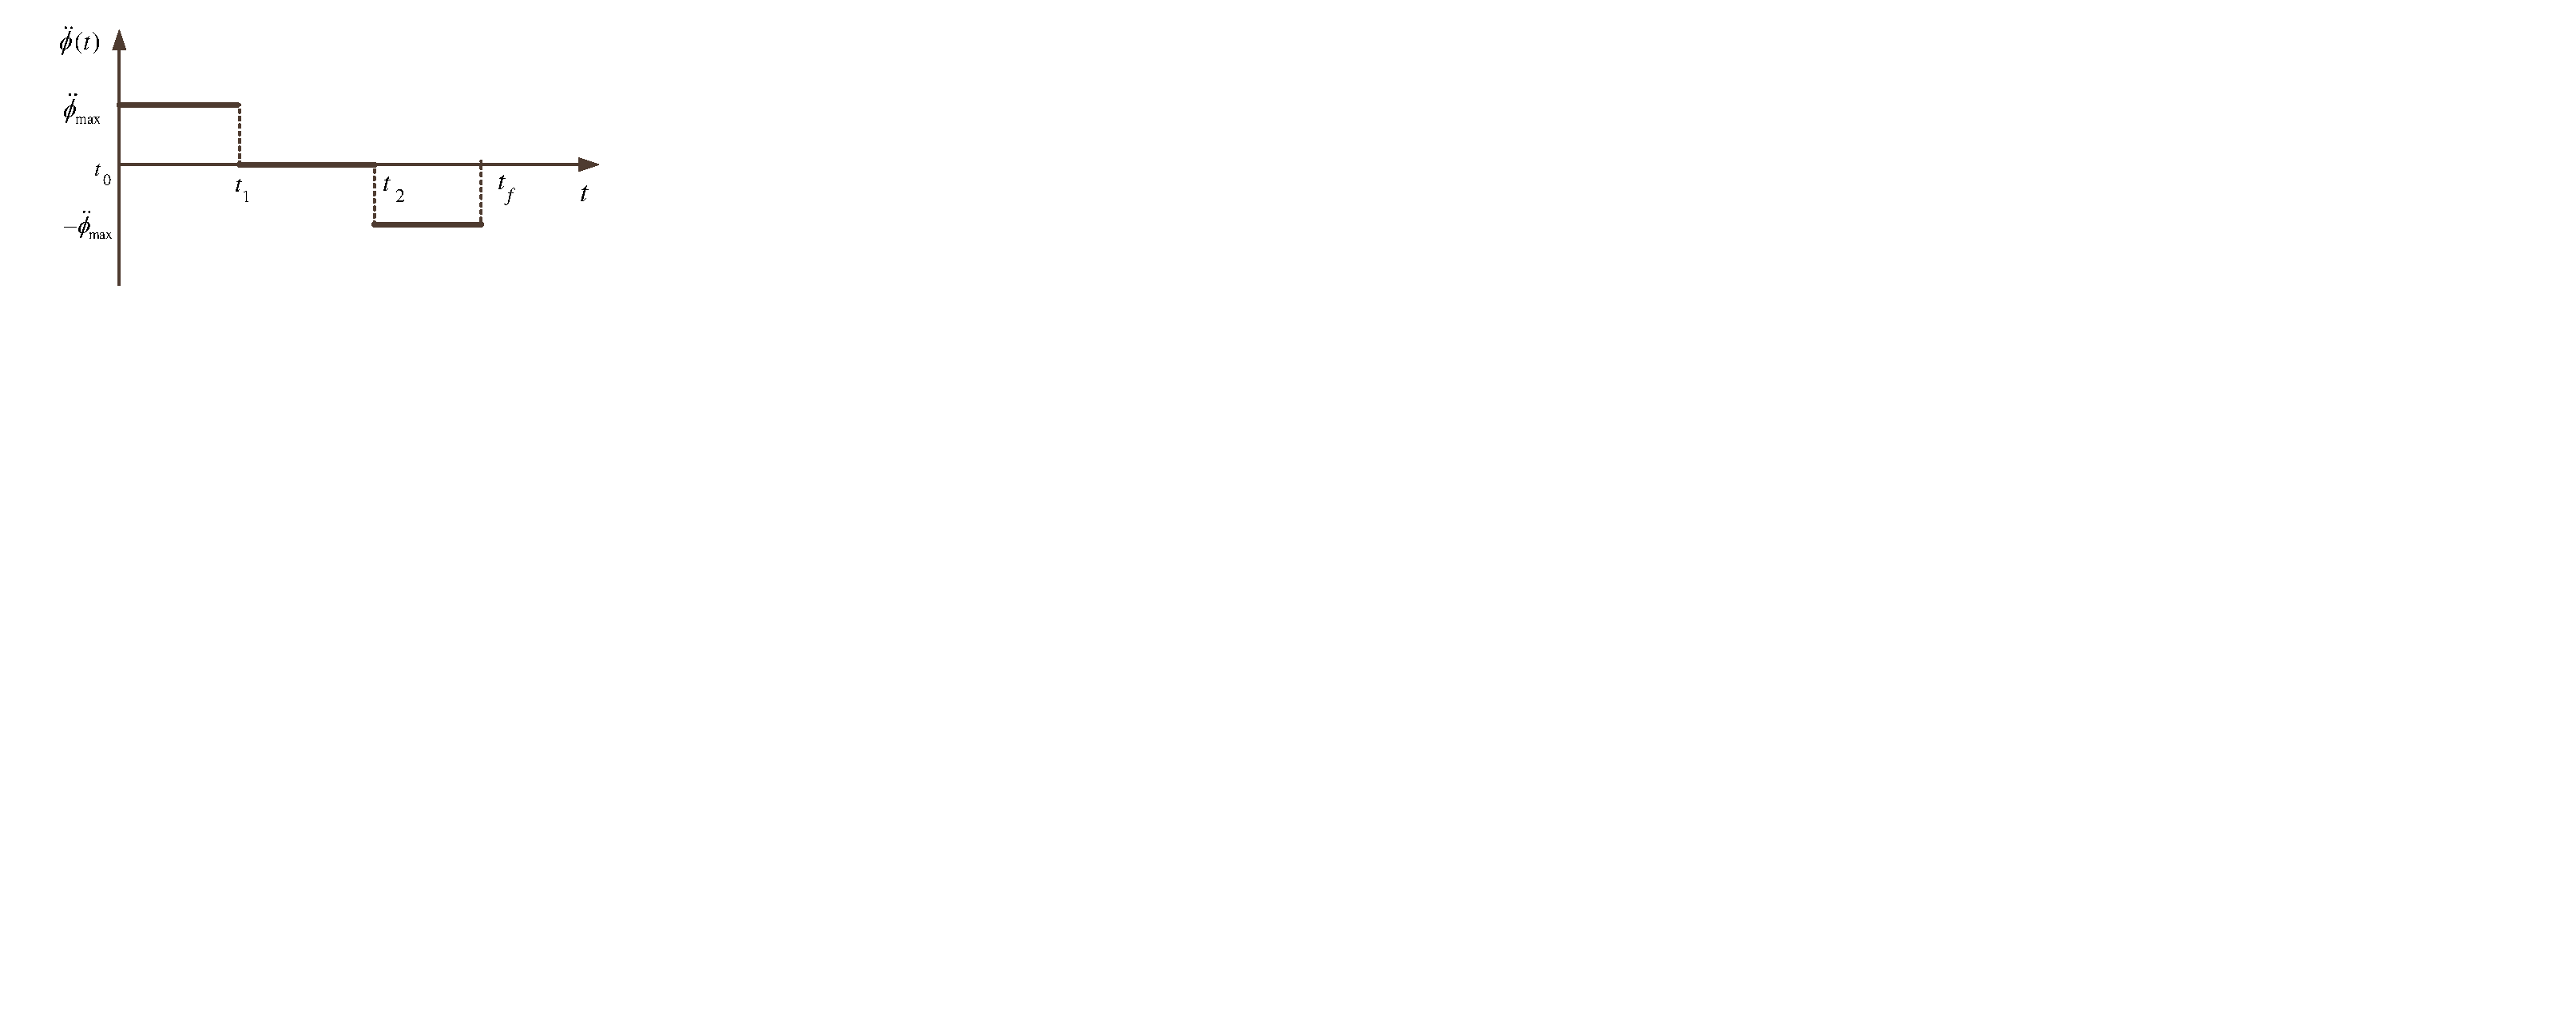
\includegraphics[width=1.5in]{./Figures/bang_off_bang}      
\end{center}
\end{minipage}
 \end{equation}
 \begin{itemize}
\item Angular velocity profile:
\end{itemize}
 \begin{equation}\label{phid_cons}
 \dot{\phi}(t)=\left\{
                \begin{array}{ll}
                \dot{\phi}_0+\ddot{\phi}_{max}(t-t_0)& when\  t_0\leq t\leq t_1,\\
                 \dot{\phi}_{max}& when\  t_1\leq t \leq t_2,\\
                 \dot{\phi}_{max}-\ddot{\phi}_{max}(t-t_2)& when \ t_2\leq t\leq t_f.
                \end{array}
              \right.
 \end{equation}
  \begin{itemize}
\item Angular position profile:
\end{itemize}
 \begin{equation}\label{phi_cons}
 \phi(t)=\left\{
                \begin{array}{ll}
                \dot{\phi}_0(t-t_0)+\frac{1}{2}\ddot{\phi}_{max}(t-t_0)^2& when\  t_0\leq t\leq t_1,\\
                \phi(t_1)+ \dot{\phi}_{max}(t-t_1)& when\  t_1\leq t \leq t_2,\\
                 \phi(t_2)+\dot{\phi}_{max}(t-t_2)-\frac{1}{2}\ddot{\phi}_{max}(t-t_2)^2& when \ t_2\leq t\leq t_f.
                \end{array}
              \right.
 \end{equation}
}
\end{block}
\end{frame}


%-------------------------------------------------------------------------------------------------------------------------------------------------------------------
\begin{frame}
\begin{block}{ Single-Axis, Agile Slew Maneuver with Velocity and Acceleration Constraints}
\begin{itemize}
\item Using the conditions, $\dot{\phi}(t_1)=\dot{\phi}_{max}$, $\dot{\phi}(t_f)=\dot{\phi}_f$, $\phi(t_f)=\phi_f$, we can determine switching times $t_1$, $t_2$, and final time $t_f$ as:
\end{itemize}
 \begin{equation}\label{t1cons}
t_1=t_0+\frac{\dot{\phi}_{max}-\dot{\phi}_0}{\ddot{\phi}_{max}},
 \end{equation}
 \begin{equation}\label{t2cons}
 \begin{split}
 t_2=&t_1+\frac{1}{\dot{\phi}_{max}}\Big[ \phi_f-\dot{\phi}_0(t_1-t_0)-\frac{1}{2}\ddot{\phi}_{max}(t_1-t_0)^2\\
 &-\frac{\dot{\phi}_{max}(\dot{\phi}_{max}-\dot{\phi}_f)}{\ddot{\phi}_{max}}+\frac{(\dot{\phi}_{max}-\dot{\phi}_f)^2}{2\ddot{\phi}_{max}} \Big],
 \end{split}
 \end{equation}
and
  \begin{equation}\label{tfcons}
 t_f=t_1+\frac{1}{\dot{\phi}_{max}}\Big[ \phi_f-\dot{\phi}_0(t_1-t_0)-\frac{1}{2}\ddot{\phi}_{max}(t_1-t_0)^2+\frac{(\dot{\phi}_{max}-\dot{\phi}_f)^2}{2\ddot{\phi}_{max}} \Big].
 \end{equation}
\end{block}
\end{frame}

%-------------------------------------------------------------------------------------------------------------------------------------------------------------------
\begin{frame}
\begin{block}{ Single-Axis, Agile Slew Maneuver with Velocity and Acceleration Constraints}
\begin{itemize}
\item Steering profiles:
\begin{equation}
^Nq^D(t)=[e_x\sin\frac{\phi(t)}{2}, e_y\sin\frac{\phi(t)}{2}, e_z\sin\frac{\phi(t)}{2}, \cos\frac{\phi(t)}{2}]^T
\end{equation}
\begin{equation}
^N_G\omega^D(t)=\dot{\phi}(t)_G\hat{e}
\end{equation}
\begin{equation}
^N_G\alpha^D(t)=\ddot{\phi}(t)_G\hat{e}
\end{equation}
\end{itemize}
\end{block}
\end{frame}

%-------------------------------------------------------------------------------------------------------------------------------------------------------------------
\begin{frame}
\begin{block}{}
\begin{center}
{\LARGE{Computing the Steering Profiles}}
\begin{itemize}
\item Case 2)  Single-Axis, Agile Slew Maneuver with Acceleration Constraint.
\end{itemize}
\end{center}
\end{block}
\end{frame}

%%%%%%%%%%%%%%%%%%%%%%%%%%%%%%%%%%%%%%%%%%%%%%%%%%%%%%%%%%%%%%
%-------------------------------------------------------------------------------------------------------------------------------------------------------------------
\begin{frame}
\begin{block}{ Single-Axis, Agile Slew Maneuver with Acceleration Constraint}
 {\bf Problem Statement:} \\ Consider the optimal control problem described by Eqs.(\ref{costfunction}), (\ref{system}), (\ref{Bcs}), and subject to control constraint
\begin{equation}
C_2: \ |u=\ddot{\phi}|\leq \ddot{\phi}_{max}.
\end{equation}
 {\bf Find:} $\phi(t)$, $\dot{\phi}(t)$, and $\ddot{\phi}(t)$.
 \end{block}
 \end{frame}

%-------------------------------------------------------------------------------------------------------------------------------------------------------------------
\begin{frame}
\begin{block}{ Single-Axis, Agile Slew Maneuver with Acceleration Constraint}

\begin{itemize}
	\item Angular acceleration about the $\hat{e}$ axis:
\end{itemize}
\begin{equation}\label{alpha}
\ddot{\phi}(t)=\ddot{\phi}_{max}\mathbb{U}(t_0)- 2\ddot{\phi}_{max}\mathbb{U}(t-t_1)
\end{equation}

\begin{center}
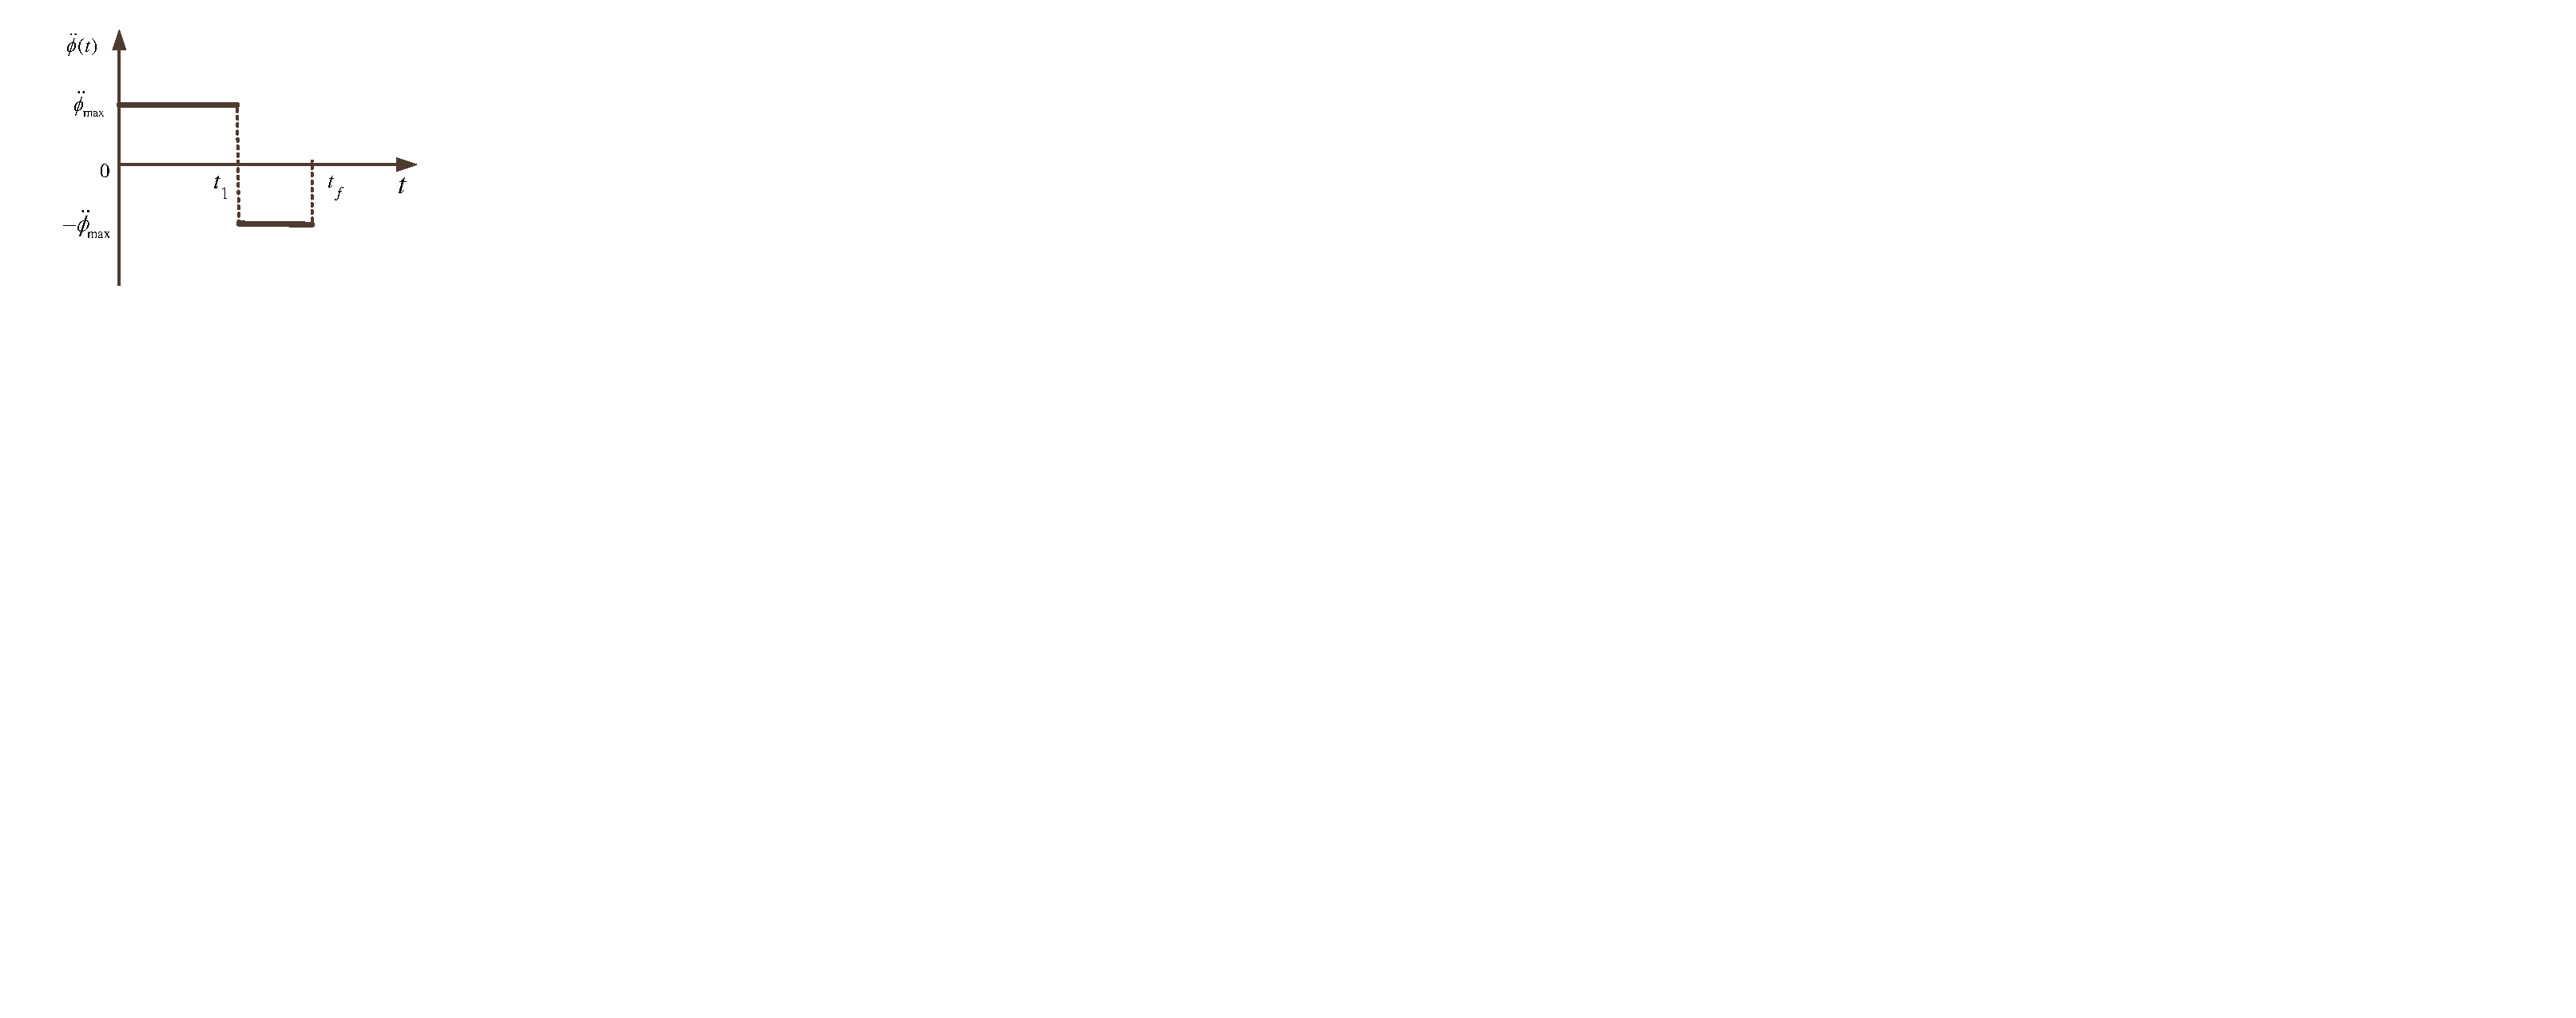
\includegraphics[width=2in]{./Figures/Bang_bang}      
\end{center}

where the switching and the final times are given by
\begin{equation}
t_1=t_0-\frac{\dot{\phi}_{0}}{\ddot{\phi}_{max}}+\frac{\sqrt{\ddot{\phi}_{max}^2(2\ddot{\phi}_{max}\phi_{f}+\dot{\phi}_{f}^2+\dot{\phi}_{0}^2)}}{\sqrt{2}\ddot{\phi}_{max}^2}
\end{equation}


\end{block}
\end{frame}
%-------------------------------------------------------------------------------------------------------------------------------------------------------------------
\begin{frame}
\begin{block}{ Single-Axis, Agile Slew Maneuver with Acceleration Constraint}
and
\begin{equation}
t_f=t_0-\frac{\dot{\phi}_{f}+\dot{\phi}_{0}}{\ddot{\phi}_{max}}+\frac{\sqrt{2}\sqrt{\ddot{\phi}_{max}^2(2\ddot{\phi}_{max}\phi_{f}+\dot{\phi}_{ef}^2+\dot{\phi}_{0}^2)}}{\ddot{\phi}_{max}^2}
\end{equation}
\begin{itemize}
	\item Angular velocity about the $\hat{e}$ axis:
\end{itemize}
\begin{equation}\label{omega}
\dot{\phi}(t)=\dot{\phi}_{0}+\ddot{\phi}_{max}(t-t_0)\mathbb{U}(t_0)- 2\ddot{\phi}_{max}(t-t_1)\mathbb{U}(t-t_1)
\end{equation}
\begin{itemize}
	\item Angular position about the $\hat{e}$ axis:
\end{itemize}
\begin{equation}\label{phi}
\begin{split}
\phi(t)&=\dot{\phi}_{0}(t-t_0)+\ddot{\phi}_{max}\frac{(t-t_0)^2}{2}\mathbb{U}(t_0)\\
&- 2\ddot{\phi}_{max}\frac{(t-t_1)^2}{2}\mathbb{U}(t-t_1)
\end{split}
\end{equation}
\end{block}
\end{frame}

%-------------------------------------------------------------------------------------------------------------------------------------------------------------------
\begin{frame}{The Agile Sun-Avoidance Slew Maneuver}
\begin{block}{The First Slew Maneuver: \\ A single-axis nonrest-to-rest maneuver around the $\hat{e}$}

\begin{itemize}
\item The BCs: 
\end{itemize}
\begin{equation}\label{Bc1}
\dot{\phi}(t_0)=\dot{\phi}_{0},\phi(t_0)=0, \dot{\phi}(t_{f1})=0,\phi(t_{f1})=\phi_1.
\end{equation}

 The switching time, $t_{11}$, and minimum-time, $t_{f1}$, are
\begin{equation}\label{t11}
t_{11}=t_0-\frac{\dot{\phi}_0}{\ddot{\phi}_{max}}+\frac{\sqrt{\ddot{\phi}_{max}^2(2\ddot{\phi}_{max}\phi_1+\dot{\phi}_{0}^2)}}{\sqrt{2}\ddot{\phi}_{max}^2}
\end{equation}
\begin{equation}\label{tf1}
t_{f1}=t_0-\frac{\dot{\phi}_0}{\ddot{\phi}_{max}}+\frac{\sqrt{2\ddot{\phi}_{max}^2(2\ddot{\phi}_{max}\phi_1+\dot{\phi}_{0}^2)}}{\ddot{\phi}_{max}^2}
\end{equation}
The $\ddot{\phi}(t)$, $\dot{\phi}(t)$, and  $\phi(t)$,  can be found by substituting the boundary conditions given by (\ref{Bc1}) and $t_{11}$ and $t_{f1}$ in to Eqs. (\ref{alpha}), (\ref{omega}), and (\ref{phi}), respectively.
\end{block}
\end{frame}
%-------------------------------------------------------------------------------------------------------------------------------------------------------------------

\begin{frame}{The Agile Sun-Avoidance Slew Maneuver}
\begin{block}{The Second Slew Maneuver: A rest-to-rest maneuver around the sun vector}
\begin{itemize}
\item The BCs: 
\end{itemize}
\begin{equation}\label{Bc2}
\dot{\phi}(t_0)=0,\phi(t_0)=0, \dot{\phi}(t_{f2})=0,\phi(t_{f2})=\phi_2.
\end{equation}
 The switching time, $t_{12}$, and the minimum-time, $t_{f2}$, are
\begin{equation}\label{t21}
t_{12}=t_0-\frac{\sqrt{\phi_2}}{\ddot{\phi}_{max}}
\end{equation}
\begin{equation}\label{tf2}
t_{f2}=t_0-\frac{2\sqrt{\phi_2}}{\ddot{\phi}_{max}}
\end{equation}
The $\ddot{\phi}(t)$, $\dot{\phi}(t)$, and  $\phi(t)$,  can be found by substituting the boundary conditions given by (\ref{Bc2}) and $t_{12}$ and $t_{f2}$ in to Eqs. (\ref{alpha}), (\ref{omega}), and (\ref{phi}), respectively.
\end{block}
\end{frame}
%-------------------------------------------------------------------------------------------------------------------------------------------------------------------

\begin{frame}{The Agile Sun-Avoidance Slew Maneuver}
\begin{block}{The Third Slew Maneuver: A single-axis rest-to-nonrest maneuver around the $\hat{e}$}
\begin{itemize}
 \item The BCs: 
\end{itemize}
\begin{equation}\label{Bc3}
\dot{\phi}(t_0)=0,\phi(t_0)=0, \dot{\phi}(t_{f3})=\dot{\phi}_{f},\phi(t_{f3})=\phi_3.
\end{equation}
 The switching time, $t_{13}$, and the minimum-time, $t_{f3}$, are
\begin{equation}\label{t31}
t_{13}=t_0+\frac{\sqrt{\ddot{\phi}_{max}^2(2\ddot{\phi}_{max}\phi_3+\dot{\phi}_{f}^2)}}{\sqrt{2}\ddot{\phi}_{max}^2}
\end{equation}
\begin{equation}\label{tf3}
t_{f3}=t_0-\frac{\dot{\phi}_{f}}{\ddot{\phi}_{max}}+\frac{\sqrt{2\ddot{\phi}_{max}^2(2\ddot{\phi}_{max}\phi_3+\dot{\phi}_{f}^2)}}{\ddot{\phi}_{max}^2}
\end{equation}
The $\ddot{\phi}(t)$, $\dot{\phi}(t)$, and  $\phi(t)$,  can be found by substituting the boundary conditions given by (\ref{Bc3}) and $t_{13}$ and $t_{f3}$ in to Eqs. (\ref{alpha}), (\ref{omega}), and (\ref{phi}), respectively.
\end{block}
\end{frame}


%%-------------------------------------------------------------------------------------------------------------------------------------------------------------------
%
%\begin{frame}
%\begin{block}{The Sun-Avoidance Slew Maneuver Procedure}
%\begin{itemize}
% \item{\bf  Data:}  $_N\hat{P}_i$, $_N\hat{P}_f$, $_N\hat{S}$, $_B\hat{P}$, $\epsilon_p$, $^Nq^B$, $^N_B\omega^B(t_i)$, $^N_B\omega^B(t_f)$, and $_Bu_M$ .\\
%\item {\bf Result:} $^N_B\omega^R(t)$, $^N_B\alpha^R(t)$,  and $^Nq^R(t)$.
%\end{itemize}
%\end{block}
%\begin{block}{}
%\begin{enumerate}
%\item Calculate the angular separation angle between the sun vector and the $\hat{P}_i-\hat{P}_f$ plane.
%\item ${\bf if}$ $|\alpha|<\epsilon_p$ {\bf then}
%\item Calculate the projection of the unit sun-vector, $\hat{S}$, on the $\hat{P}_i-\hat{P}_f$ plane, $_N\hat{S}_{||}$ from Eq.(\ref{Sbar}).
%\item Use the $^Nq^B$ to find the direction cosine matrix, $^NC^B$ and from there find $_B\hat{S}_{||}$.
%\item Calculate the first rotation angle, $\phi_1$ from Eq.(\ref{phi1}), the first rotation axis vector, $e$, from Eq.(\ref{eaxis}), and from there $^Nq^R$.
%\item Calculate $\ddot{\phi}_{max}=_Bu_M^{T}\ ^BC^N \ _Ne$.
%\seti
%\end{enumerate}
%\end{block}
%\end{frame}
%%-------------------------------------------------------------------------------------------------------------------------------------------------------------------
%\begin{frame}
%\begin{block}{The Sun-Avoidance Slew Maneuver Procedure- Continued}
%%\begin{itemize}
%\begin{enumerate}
%\conti
%\item Calculate $\alpha_e(t)=^N_N\alpha^R(t)$, $\omega_e(t)=^N_N\omega^R(t)$, and  $\phi_e(t)$, from Eqs. (\ref{alpha}), (\ref{omega})--(\ref{tf1}), respectively.
%\item Calculate the angular velocity and angular acceleration profiles in the body-fixed frame. i.e. $ ^N_N\omega^R\rightarrow ^N_B\omega^R$ and $^N_N\alpha^R\rightarrow ^N_B\alpha^R$.
%\item Calculate the second rotation angle, $\phi_2$, from Eq.(\ref{phi2}), and using the unit sun-vector $\hat{S}$, $^Nq^R$.
%\item Calculate $\ddot{\phi}_{max}=_Bu_M^{T}\ ^BC^N \ _NS$.
%\item Calculate $\alpha_e(t)=^N\alpha_N^R(t)$, $\omega_e(t)=^N\omega_N^R(t)$, and  $\phi_e(t)$ from Eqs. (\ref{alpha}), (\ref{omega})--(\ref{phi}), (\ref{t21}), and (\ref{tf2}), respectively.
%\item Calculate the angular velocity and angular acceleration profiles in the body-fixed frame. i.e. $^N_N\omega^R\rightarrow ^N_B\omega^R$ and $^N_N\alpha^R\rightarrow ^N_B\alpha^R$.
%\item Calculate the third rotation angle, $\phi_3$, from Eq.(\ref{phi3}), and using the unit vector $\hat{e}$ to calculate $^Nq^R$.
%\seti
%\end{enumerate}
%%\end{itemize}
%\end{block}
%\end{frame}
%
%%-------------------------------------------------------------------------------------------------------------------------------------------------------------------
%\begin{frame}
%\begin{block}{The Sun-Avoidance Slew Maneuver Procedure- Continued}
%%\begin{itemize}
%\begin{enumerate}
%\conti
%\item Calculate $\ddot{\phi}_{max}=_Bu_M^{T}\ ^BC^N \ _Ne$.
%\item Calculate $\alpha_e(t)=^N\alpha_N^R(t)$, $\omega_e(t)=^N\omega_N^R(t)$, and  $\phi_e(t)$ from Eqs. (\ref{alpha}), (\ref{omega})--(\ref{phi}), (\ref{t31}), and (\ref{tf3}), respectively.
%\item Calculate the angular velocity and angular acceleration profiles in the body-fixed frame. i.e. $^N_N\omega^R\rightarrow ^N_B\omega^R$ and $^N_N\alpha^R\rightarrow^N_B\alpha^R$.
%\item Perform the final slew rotation around the instrument boresight axis via angle $\phi_4$
%\item ${\bf else}$
%\item Perform the regular slew maneuver.
%\item  ${\bf end}$
%\end{enumerate}
%%\end{itemize}
%\end{block}
%\end{frame}
%%-------------------------------------------------------------------------------------------------------------------------------------------------------------------
%\begin{frame}
%\begin{block}{Calculating $\omega_c$, and $\alpha_c$}
%\begin{itemize}
%\item Assumptions:
%%A1: Using the first-order approximation.\\
%%A2: $ \omega$ is constant during each step.
%%\begin{equation}
%%\begin{split}
%%\begin{bmatrix} \omega_1(k)\\ \omega_2(k)\\ \omega_3(k)\end{bmatrix}\approx &\frac{2}{\Delta t}\begin{bmatrix}q_4(k)&q_3(k)&-q_2(k)&-q_1(k)\\-q_3(k)&q_4(k)&q_1(k)&-q_2(k)\\q_2(k)&-q_1(k)&q_4(k)&-q_3(k)\end{bmatrix}\times\\
%%&\begin{bmatrix}\ q_1(k+1)-q_1(k)\\ q_2(k+1)-q_2(k)\\ q_3(k+1)-q_3(k)\\ q_4(k+1)-q_4(k)\end{bmatrix}
%%\end{split}
%% \end{equation}
%%and 
%%\begin{equation}
%%\begin{bmatrix} \alpha_1(k)\\ \alpha_2(k)\\ \alpha_3(k)\end{bmatrix}\approx\frac{1}{\Delta t}\begin{bmatrix} \omega_1(k+1)-\omega_1(k)\\ \omega_2(k+1)-\omega_2(k)\\ \omega_3(k+1)-\omega_3(k)\end{bmatrix}
%%\end{equation}
%\end{itemize}
%\end{block}
%\end{frame}
\end{document}


